% --- ARCHITETTURE DEGLI ELABORATORI ---
\documentclass[a4paper, 12pt]{article} % Qui era 12pt

% --- PACKAGES ---

\usepackage[italian]{babel}
\usepackage{comment}

\usepackage{microtype}
\usepackage{graphicx}
\usepackage{wrapfig}
\usepackage{enumitem}
\usepackage{fancyhdr}

\usepackage{amsmath}

%\usepackage{paralist} % SE ATTIVO PARALIST, ITEMIZE ED ENUMERATE NON FUNZIONANO!!!

\usepackage{amsthm}
% it introduces the \newtheorem command
\usepackage{amssymb}
% new mathematical symbols
\usepackage{eucal}
% other mathematical symbols
\usepackage{gensymb}
% \degree \celsius \micro \ohm \perthousand
\usepackage{mathptmx}
% other mathematical symbols
\usepackage{latexsym}
% other mathematical symbols
\usepackage{mathtools}
% supplements amsmath
\usepackage{textcomp}
% extra symbols arrows like \textrightarrow, \texteuro, \textcelsius

\usepackage[utf8]{inputenc}

\usepackage{multicol}
% Per le colonne

%\usepackage{xcolor}
% Per colorare il testo

\usepackage[table, dvipsnames]{xcolor}
% Per ulteriori colori
% Quel table serve invece per colorare le righe in tabular

\usepackage[document]{ragged2e}

\usepackage{blindtext}

\usepackage[scaled=.92]{helvet}

\usepackage{tikz}

%\usepackage{floatrow}

%\usepackage{makecell}

\usepackage[T1]{fontenc}
%\usepackage{fourier, erewhon}
%\usepackage{geometry}
\usepackage{array, caption, floatrow, tabularx, makecell, booktabs}%

\usepackage{amsfonts}

%\graphicspath{ {./images/} }
% graphicspath dice a LaTex la path della cartella dove si trovano le immagini.

%\usepackage{float}

\usepackage{etoc}

\usepackage{titlesec}
%\titleformat{\section}{\normalfont\Large\bfseries\center}{}{0pt}{} % Questo serve per togliere il numero dalla section ; Qui ho aggiunto \center e ora sono centrati

\usetikzlibrary{snakes}

\usepackage[most]{tcolorbox}

%\begin{comment}

\titleformat
{\section} % command
[display] % shape
{\normalfont\Large\bfseries\center} % format
{} % label
{-2ex} % sep %0.5ex
{
	\rule{\textwidth}{1pt} % 1 pt
	\vspace{-2pt} % 1ex
	\centering
} % before-code
[
\vspace{-2ex}% -0.5ex valori originari
\rule{\textwidth}{0.3pt} % 0.3pt
] % after-code

%\end{comment}

\begin{comment}
\titleformat{\section}[block]
{\titlerule\addvspace{4pt}\normalfont\Large\bfseries\center}
{\thesection\enspace}{0pt}{}[\vspace{2pt}\titlerule]
\end{comment}

\titleformat{\subsection}{\normalfont\Large\bfseries\center\color{red}}{}{0pt}{} % Questo l'ho copiato da sopra ed ho aggiunto center e ora sono centrati
\titleformat{\subsubsection}{\normalfont\Large\bfseries\center\color{red}}{}{0pt}{} % Questo l'ho copiato da sopra ed ho aggiunto center e ora sono centrati
\setcounter{secnumdepth}{1} % levels under \section are not numbered
\setcounter{tocdepth}{2}    % levels under \subsection are not listed in the TOC

%\usepackage{sectsty} % Se lo attivo mi metti i numerini nella section
%\sectionfont{\centering}
%\allsectionsfont{\centering}

\usepackage{diffcoeff} % per le derivate

\usepackage{lipsum}

\usepackage{ltablex}

%\usepackage{multirow}

%\usepackage{systeme}

\usetikzlibrary{arrows.meta}

\usetikzlibrary{chains,decorations.pathreplacing}

\usepackage[normalem]{ulem} % serve per sbarrare il testo (strikethrough), usare \sout

\usetikzlibrary{tikzmark} % per circondare gli elementi di una tabella (tabular)

\usetikzlibrary{shapes}

\usepackage{circuitikz}

\usetikzlibrary{arrows,shapes.gates.logic.US,shapes.gates.logic.IEC,calc}

\tikzstyle{branch}=[fill,shape=circle,minimum size=3pt,inner sep=0pt]

\usepackage{subfig} % serve per avere immagini una accanto all'altra

\usepackage{cancel} 

\usetikzlibrary{matrix}

\usepackage{soul}

%\usepackage{emerald}% per dalla 1-4 firma (questo mi da errore, not found)

\usepackage{frcursive}% serve per la firma finale (nelle Conclusioni)

\usepackage{inslrmin}% per la 6 firma

% !TeX root = ../Architetture_Degli_Elaboratori.tex

% --- FINE USEPACKAGES ---

\makeindex

\begin{document}

\title{\huge{\textbf{Architetture degli Elaboratori}}}
\author{Luca}
\date{14, Novembre 2020}

\maketitle	

\pagebreak

% INIZIO: TABLEOFCONTENTS

\let\cleardoublepage\clearpage
\tableofcontents
\pagenumbering{arabic}
\setcounter{page}{2}
%\etocsettocstyle{\subsection*{This Chapter contains:}}{\noindent\rule{\linewidth}{.4pt}}
% C'è bisogno del package etoc
%\chapter{Extinct Species}
%\localtableofcontents

% FINE: TABLEOFCONTENTS

\fancyhf{}
\begin{comment}
\renewcommand{\headrulewidth}{2pt}
\renewcommand{\footrulewidth}{1pt}
\fancyhead[LE]{\leftmark}
\fancyhead[RO]{\nouppercase{\rightmark}}
\fancyfoot[LE, RO]{\thepage}
\end{comment}

% --- CONVERSIONE BINARIO, OTTALE, DECIMALE, ESADECIMALE ---

\newpage

\section{Conversione Binario - Ottale - Decimale - Esadecimale}


\textsf{\large{\color{red} Esercizi: 1) Convertire i seguenti numeri decimali in \
		base 2: $371, 3224, 114.65625$}} \\

$\mathbf{371} = 2^8 + 115 \rightarrow 115 = 2^6 + 51 \rightarrow 51 = 2^5 + 19$ $\rightarrow 19 = 2^4 + 3$ \\ $3 = 2^1 + 1 \rightarrow 1 = 2^0 $ \\
$ 2^8 + 2^6 + 2^5 + 2^4 + 2^1 + 2^0 = \mathbf{371} $ \\
$ \mathbf{371_{10}} = 101110011_2 $ \hspace{0.3cm} \textrm{\color{red} METODO 1}
\\
\textrm{\color{red} METODO 2} \\

\noindent\begin{minipage}{.25\linewidth}
\begin{equation*}
\begin{tabular}{c|c}
371 & \\
185 & 1 \\
92 & 1 \\
46 & 0 \\
23 & 0 \\
11 & 1 \\
5 & 1 \\
2 & 1 \\
1 & 0 \\
0 & 1
\end{tabular}
\end{equation*}
\end{minipage}
\begin{minipage}{.25\linewidth}
\textrm{\color{red}\textuparrow \hspace{0.2cm}Dal basso verso l'Alto} \\
$ \mathbf{371_{10} = 101110011_2}$ \\
\end{minipage}
\quad

% --- 3224 ---
\textrm{\color{red} 3224} \\
\noindent\begin{minipage}{.25\linewidth}
\begin{equation*}
	\begin{tabular}{c|c}
		3224 & \\
		1612 & 0 \\
		806 & 0 \\
		403 & 0 \\
		201 & 1 \\
		100 & 1 \\
		50 & 0 \\
		25 & 0 \\
		12 & 1 \\
		6 & 0 \\
		3 & 0 \\
		1 & 1 \\
		0 & 1
	\end{tabular}
\end{equation*}
\end{minipage}
\begin{minipage}{.25\linewidth}
$ \mathbf{3224_{10} = 110010011000_2} $ \\
\end{minipage}
\quad

% --- 114,65625 ---
\pagebreak
\textrm{\color{red} 114,65625} \\
\begin{align*}
	114,65625 &= 2^6 + 50,65625 \\
	50,65625 &= 2^5 + 18,65625 \\
	18,65625 &= 2^4 + 2,65625 \\
	2,65625 &= 2^1 + 0,65625 \\
	0,65625 &= 2^{-1} + 0,15625 \\
	0,15625 &= 2^{-3} + 0,03125 \\
	0,03125 &= 2^{-5} \\
\end{align*}

\centering{
$ \mathbf{114,65625_{10} = 1110010,10101_2} $
}

% --- ESERCIZIO 2 ---
\flushleft{
\textsf{\large{\color{red} 2) Convertire i seguenti numeri in base 8 e 16}} \\
}

\begin{gather*}
	\underbrace{\rm 11} \hspace{0.3cm}\underbrace{100} \hspace{0.3cm} \underbrace{110} \hspace{0.3cm} \underbrace{100} \hspace{0.3cm} \underbrace{110}\\
	\hspace{0.5cm}2^1 + 2^0 \hspace{0.5cm}4 \hspace{0.7cm} 6 \hspace{1cm} 2^2 \hspace{0.7cm} 2^2 + 2^1
\end{gather*}

\textsf{\normalsize{Raggruppo in gruppi di 3 (questo per la base 8) $ 8 \text{ è } 2^3$}} \\
$ \mathbf{11100110100110_2 = 34646_8} $ \\

\begin{gather*}
	\underbrace{\rm 11} \hspace{0.3cm}\underbrace{1001} \hspace{0.3cm} \underbrace{1010} \hspace{0.3cm} \underbrace{0110} \\
	\hspace{0.5cm}2^1 + 2^0 \hspace{0.5cm}9 \hspace{0.5cm}10 = A \hspace{0.5cm} 2^2 + 2^1
\end{gather*}

\textsf{\normalsize{Raggruppo in gruppi di 4 (questo per la base 16) $ 16 \text{ è } 2^4$}} \\
$ \mathbf{11100110100110_2 = 39A6_{16}} $ \break

% --- ESERCIZIO 3 ---

\textsf{\large{\color{red} 3) Convertire i numeri esadecimali in binario}} \\

$ \color{red}\boxed{\normalcolor F} \color{blue}\boxed{\normalcolor A} \color{green}\boxed{\normalcolor 3} \color{violet}\boxed{\normalcolor 1} \color{orange}\boxed{\normalcolor C}$ \textsf{\normalsize{Una cifra può essere rappresentata da 4 cifre binarie}} \\

\begin{align*}
	\color{red}15_{10} &= 2^3 + 2^2 + 2^1 + 2^0 = 1111_2 \\
	\color{blue}A_{16} &= 10_{10} = 2^3 + 2^1 = 1010_2 \\
	\color{green}3_{16} &= 3_{10} = 2^1 + 2^0 = 0011_2 \\
	\color{violet}1_{16} &= 1_{10} = 2^0 = 0001_2 \\
	\color{orange}C_{16} &= 12_{10} = 2^3 + 2^2 = 1100_2 \\
\end{align*}

$\mathbf{FA31C_{16} = 11111010001100011100_2}$ \\

% --- ESERCIZIO 4 ---

\textsf{\large{\color{red} 4) Convertire da esadecimale a decimale}} \\

$ AAB_{16} $ \\

\begin{align*}
	B \cdot 16^0 &= 11 \cdot 1 = 11 \\
	A \cdot 16^1 &= 10 \cdot 16 = 160 \\
	A \cdot 16^2 &= 10 \cdot 256 = 2560 \\
\end{align*}

$ 12 + 160 + 2560 = 2731 $ \\
$ \mathbf{AAB_{16} = 2731_{10}} $ \\

% --- COMPLEMENTO A 2, ECCESSO 128 E 256, MASCHERATURE DEI BITS ---

\newpage

\section{Complemento a 2 - Eccesso 128 e 256 - Mascherature dei bits}

\textsf{\large{\color{red} 5) \textbf{\normalcolor Quanti valori sono codificabili con 2-4-7-10 bit?}}} \\

\textsf{\normalsize{$N$ bit $ \Longrightarrow 2^N$}} \break

\textsf{\large{\color{red} 6) \textbf{\normalcolor Per codificare 1598 numeri quanti bit/byte sono necessari?}}} \\

$ 2^N \geq 1598 $ \\ $ 2^{10} = 1024 $ \\ $ 2^{11} = 2048 > 1598 $ \\
$2$ \text{ byte } = $16$ \text{ bit } \\
\textsf{\normalsize{Il byte o lo si prende tutto o niente.}} \\

$ 2^{16} = 65536 > 1598 $ \break

\textsf{\large{\color{red} 7) \textbf{\normalcolor Quante cifre binarie sono necessarie per codificare X numeri distinti ($log_2 X = log_{10} X / log_{10} 2$)?}}} \break

\textsf{\large{\color{red} 8) \textbf{\normalcolor Si convertono i seguenti numeri decimali in numeri binari in complemento a 2: $-56, -88, 243$ Si utilizzino 8 bit per rappresentare il risultato?}}} \break

\textsf{\large{\color{red} 9) \textbf{\normalcolor Si convertano i seguenti numeri decimali in numeri binari in eccesso 128 e 256. $-56, -37, -243$}}} \break

% --- ESERCIZIO 10 ---

\textsf{\large{\color{red} 10) \textbf{\normalcolor Si pongano a 1 bit di posizione dspari del byte. $11010011$}}} \\

\newcommand{\AND}{\text{\textrm{\color{red}{AND}}}}
\newcommand{\OR}{\text{\textsl{\color{red}{OR}}}}
%\newcommand{\sumOut}{\text{\textsl{\color{gray}{Sum}}}}

\noindent\begin{minipage}{.5\linewidth}
\begin{equation*}
	\begin{tikzpicture}[
		row 1/.style={font=\textsl,font=\scriptsize,black!85, anchor=west,
			inner sep=1.5pt},
		every node/.style={column sep=.5mm,row sep=1mm}]
		\matrix (m) [matrix of math nodes,
		nodes in empty cells,
		%nodes=draw
		] 
		{
			&   &   &   &   &   &   &   &   &\\
			& 1 & 1 & 0 & 1 & 0 & 0 & 1 & 1 & \\    
			& 1 & 0 & 1 & 0 & 1 & 0 & 1 & 0 &[10mm]		\OR  \\ 
			& 1 & 1 & 1 & 1 & 1 & 0 & 1 & 1 & \\                                          
		};
	
		\draw[-,color=black,semithick] (m-3-2.south west) -- (m-3-9.south east);
	\end{tikzpicture}
\end{equation*}
\end{minipage}
\quad
\begin{minipage}{.25\linewidth}
\begin{tabular}{c|c|c}
	A & B & A OR B \\
	\hline
	0 & 0 & 0 \\
	0 & 1 & 1 \\
	1 & 0 & 1 \\
	1 & 1 & 1 \\
\end{tabular}
\quad
\end{minipage}
\textsf{\normalsize{\\Poteva andare bene anche questa mascheratura: }} \\
\begin{minipage}{.5\linewidth}
\begin{equation*}
	\begin{tikzpicture}[
		row 1/.style={font=\textsl,font=\scriptsize,black!85, anchor=west,
			inner sep=1.5pt},
		every node/.style={column sep=.5mm,row sep=1mm}]
		\matrix (m) [matrix of math nodes,
		nodes in empty cells,
		%nodes=draw
		] 
		{
			&   &   &   &   &   &   &   &   &\\
			& 1 & 1 & 0 & 1 & 0 & 0 & 1 & 1 & \\    
			& 0 & 0 & 1 & 0 & 1 & 0 & 0 & 0 &[10mm]		\OR  \\ 
			& 1 & 1 & 1 & 1 & 1 & 0 & 1 & 1 & \\                                          
		};
		
		\draw[-,color=black,semithick] (m-3-2.south west) -- (m-3-9.south east);
	\end{tikzpicture}
\end{equation*}
\quad
\end{minipage}

% --- ESERCIZIO 11 ---

\textsf{\large{\color{red} 11) \textbf{\normalcolor Si pongano a 0 i primi 4 bit del byte. $11010011$}}} \\

\noindent\begin{minipage}{.5\linewidth}
\begin{equation*}
	\begin{tikzpicture}[
		every node/.style={column sep=.5mm,row sep=1mm}]
		\matrix (m) [matrix of math nodes,
		nodes in empty cells,
		%nodes=draw
		] 
		{
			& 1 & 1 & 0 & 1 & 0 & 0 & 1 & 1 & \\    
			& 0 & 0 & 0 & 0 & 0 & 0 & 1 & 1 &[10mm]		\AND  \\ 
			& 0 & 0 & 0 & 0 & 0 & 0 & 1 & 1 & \\                                          
		};
		
		\draw[-,color=black,semithick] (m-2-2.south west) -- (m-2-9.south east);
	\end{tikzpicture}
\end{equation*}
\end{minipage}
\begin{comment}
\begin{minipage}{.25\linewidth}
	\begin{tabular}{c|c|c}
		A & B & A AND B \\
		\hline
		0 & 0 & 0 \\
		0 & 1 & 0 \\
		1 & 0 & 0 \\
		1 & 1 & 1 \\
	\end{tabular}
\end{minipage}
\end{comment}
\begin{minipage}{.5\linewidth}
\begin{equation*}
	\begin{tikzpicture}[
		every node/.style={column sep=.5mm,row sep=1mm}]
		\matrix (m) [matrix of math nodes,
		nodes in empty cells,
		%nodes=draw
		] 
		{
			& 1 & 1 & 0 & 1 & 0 & 0 & 1 & 1 & \\    
			& 0 & 0 & 0 & 0 & 1 & 1 & 1 & 1 &[10mm]		\AND  \\ 
			& 0 & 0 & 0 & 0 & 0 & 0 & 1 & 1 & \\                                          
		};
		
		\draw[-,color=black,semithick] (m-2-2.south west) -- (m-2-9.south east);
	\end{tikzpicture}
\end{equation*}
\end{minipage} % è importante non aggiungere una riga, altrimenti si incasina, non so perchè
\begin{minipage}{.25\linewidth}
\begin{tabular}{c|c|c}
	A & B & A AND B \\
	\hline
	0 & 0 & 0 \\
	0 & 1 & 0 \\
	1 & 0 & 0 \\
	1 & 1 & 1 \\
\end{tabular}
\end{minipage}
\quad

\textsf{\normalsize{I primi 4 bit da sinistra o da destra? Qui l'abbiamo fatto in entrambi i modi.}} \break

% --- ESERCIZIO 12 ---

\textsf{\large{\color{red} 12) \textbf{\normalcolor Si verifichi che il terzo bit del byte $11001100$ è 1.}}} \\

\noindent\begin{minipage}{.5\linewidth}
\begin{equation*}
	\begin{tikzpicture}[
		row 1/.style={font=\textsl,font=\scriptsize,black!85, anchor=west,
			inner sep=1.5pt},
		every node/.style={column sep=.5mm,row sep=1mm}]
		\matrix (m) [matrix of math nodes,
		nodes in empty cells,
		%nodes=draw
		] 
		{
			& 7 & 6 & 5 & 4 & 3 & \color{red}2 & 1 & 0 &\\
			& 1 & 1 & 0 & 0 & 1 & 1 & 0 & 0 & \\    
			& 0 & 0 & 0 & 0 & 0 & 1 & 0 & 0 &[10mm]		\AND  \\ 
			& 0 & 0 & 0 & 0 & 0 & 1 & 0 & 0 & \\                                          
		};
		
		\draw[-,color=black,semithick] (m-3-2.south west) -- (m-3-9.south east);
	\end{tikzpicture}
\end{equation*}
\end{minipage}
\begin{minipage}{.25\linewidth}
\textsf{\normalsize{Il terzo bit a sinistra sarebbe quello in posizione \color{red}2 \normalcolor(in rosso)}} \\
\end{minipage}
\quad
\begin{minipage}{.25\linewidth}
\textsf{\normalsize{Controllo tra risultato e input}} \\
\end{minipage}
\begin{minipage}{.5\linewidth}
\begin{equation*}
	\begin{tikzpicture}[
		every node/.style={column sep=.5mm,row sep=1mm}]
		\matrix (m) [matrix of math nodes,
		nodes in empty cells,
		%nodes=draw
		] 
		{
			& 1 & 1 & 0 & 0 & 1 & 1 & 0 & 0 & \\    
			& 0 & 0 & 0 & 0 & 0 & 1 & 0 & 0 &[10mm]		\OR  \\ 
			& 1 & 1 & 0 & 0 & 1 & 1 & 0 & 0 & \\                                          
		};
		
		\draw[-,color=black,semithick] (m-2-2.south west) -- (m-2-9.south east);
	\end{tikzpicture}
\end{equation*}
\end{minipage}

% --- ESERCIZIO 13 ---

\textsf{\large{\color{red} 13) \textbf{\normalcolor Si eseguano le seguenti somme in base 2: $12_{10} + 7_{10} \hspace{0.3cm} 67_{10} + 38_{10} \hspace{0.3cm} 89_{10} + 147_{10}$}}} \\

\noindent\begin{minipage}{.25\linewidth}
\begin{align*}
	12 &= 2^3 + 2^2 \\
+	7 &= 2^2 + 2^1 + 2^0 \\
	19&
\end{align*}
\end{minipage}
\begin{minipage}{.25\linewidth}
	\begin{equation*}
		\begin{tikzpicture}[
			every node/.style={column sep=.5mm,row sep=1mm}]
			\matrix (m) [matrix of math nodes,
			nodes in empty cells,
			%nodes=draw
			] 
			{
				&   & 1 & 1 & 0 & 0 & \\    
				&   &   & 1 & 1 & 1 &[10mm]		+\\ 
				& 1 & 0 & 0 & 1 & 1 & = 2^4 + 2^1 + 2^0 = 16 + 2 + 1 = \mathbf{19}\\                                          
			};
			
			\draw[-,color=black,semithick] (m-2-2.south west) -- (m-2-6.south east);
		\end{tikzpicture}
	\end{equation*}
\end{minipage}

\pagebreak

\noindent\begin{minipage}{.25\linewidth}
\begin{align*}
	67 &+ 38 = 105 \\
	67 &= 2^6 + 2^1 + 2^0 \\
	38 &= 2^5 + 2^2 + 2^1 \\
\end{align*}
\end{minipage}
\begin{minipage}{.25\linewidth}
	\begin{equation*}
		\begin{tikzpicture}[
			every node/.style={column sep=.5mm,row sep=1mm}]
			\matrix (m) [matrix of math nodes,
			nodes in empty cells,
			%nodes=draw
			] 
			{
				& 1 & 0 & 0 & 0 & 0 & 1 & 1 &\\    
				& 0 & 1 & 0 & 0 & 1 & 1 & 0 &[10mm]		+\\ 
				& 1 & 1 & 0 & 1 & 0 & 0 & 1 & = 2^6 + 2^5 + 2^3 + 2^0 = 64 + 32 + 8 + 1 = \mathbf{105} \\                                          
			};
			
			\draw[-,color=black,semithick] (m-2-2.south west) -- (m-2-8.south east);
		\end{tikzpicture}
	\end{equation*}
\end{minipage}

\noindent\begin{minipage}{.25\linewidth}
	\begin{align*}
		89 &+ 147 = 236 \\
		89 &= 2^6 + 2^4 + 2^3 + 2^0 \\
		147 &= 2^7 + 2^4 + 2^2 + 2^0 \\
	\end{align*}
\end{minipage}
\begin{minipage}{.25\linewidth}
	\begin{equation*}
		\begin{tikzpicture}[
			every node/.style={column sep=.5mm,row sep=1mm}]
			\matrix (m) [matrix of math nodes,
			nodes in empty cells,
			%nodes=draw
			] 
			{
				&   & 1 & 0 & 1 & 1 & 0 & 0 & 1 &\\    
				& 1 & 0 & 0 & 1 & 0 & 0 & 1 & 1 &[10mm]		+\\ 
				& 1 & 1 & 1 & 0 & 1 & 1 & 0 & 0 & \\                                         
			};
			
			\draw[-,color=black,semithick] (m-2-2.south west) -- (m-2-9.south east);
		\end{tikzpicture}
	\end{equation*}
\end{minipage}

$ = 2^7 + 2^6 + 2^5 + 2^3 + 2^2 = 128 + 64 + 32 + 8 + 4 = \mathbf{236} $ \break

% --- ESERCIZIO 14 --- 

\textsf{\large{\color{red} 14) \textbf{\normalcolor Si eseguano le seguenti differenze in base 2 (complemento a 2, utilizzando 8 bit per rappresentare i numeri): $8_{10} - 17_{10} \hspace{0.3cm} 37_{10} - 23_{10} \hspace{0.3cm} 5_{10} - 117_{10}$}}} \\

\begin{itemize}
\item \textsf{\normalsize{Complemento a due:}}
	\begin{itemize}
	\item Il riporto dei bit più a sinistra viene ignorato.
	%\end{itemize}
%\end{itemize}
%\begin{itemize}
	\item \textsf{\normalsize{8 bit $[-128; +127]$}}
	%\begin{itemize}
		\item Se gli addendi sono di segno opposto non si può verificare un \
		overflow.
		\item L' \color{red} overflow \normalcolor si verifica se il riporto \
		generato è diverso dal riporto utilizzato.
		Insomma se i primi due bit a sinistra sono diversi, c'è un overflow.
	\end{itemize}
%\end{itemize}
\end{itemize}
\noindent\begin{minipage}{.25\linewidth}
\begin{align*}
&8 - 17 = -9 \Longrightarrow 8 + (-17) \\
&8 = 2^3 = \color{violet}000001000 \\
-1&7 \rightarrow 17 = 2^4 + 2^0 = \color{blue}00010001 \\
\end{align*}
\end{minipage}
\begin{minipage}{.5\linewidth}
\textsf{\normalsize{Ora invertiamo i \color{blue}bits \normalcolor del 17 e li sommiamo ad 1 (quelli in \color{blue}blu)}} \\
\end{minipage}
\noindent\begin{minipage}{.5\linewidth}
	\begin{equation*}
		\begin{tikzpicture}[
			every node/.style={column sep=.5mm,row sep=1mm}]
			\matrix (m) [matrix of math nodes,
			nodes in empty cells,
			%nodes=draw
			] 
			{
				& 1 & 1 & 1 & 0 & 1 & 1 & 1 & 0 &\\    
				&   &   &   &   &   &   &   & 1 &[10mm]		+\\ 
				& \color{orange}1 & \color{orange}1 & \color{orange}1 & \color{orange}0 & \color{orange}1 & \color{orange}1 & \color{orange}1 & \color{orange}1 & \\                                         
			};
			
			\draw[-,color=black,semithick] (m-2-2.south west) -- (m-2-9.south east);
		\end{tikzpicture}
	\end{equation*}
\end{minipage}
% Il riporto lo scrivo in verde, mentre il segno lo scrivo in rosso.
\begin{minipage}{.25\linewidth}
	\begin{equation*}
		\begin{tikzpicture}[
			row 1/.style={font=\textsl,font=\scriptsize,black!85, anchor=west,
				inner sep=1.5pt},
			every node/.style={column sep=.5mm,row sep=1mm}]
			\matrix (m) [matrix of math nodes,
			nodes in empty cells,
			%nodes=draw
			] 
			{
				\color{green}0& \color{green}0 & 0 & 0 & 1 & 0 & 0 & 0 &   &\\
				& \color{violet}0 & \color{violet}0 & \color{violet}0 & \color{violet}0 & \color{violet}1 & \color{violet}0 & \color{violet}0 & \color{violet}0 & \\    
				& \color{orange}1 & \color{orange}1 & \color{orange}1 & \color{orange}0 & \color{orange}1 & \color{orange}0 & \color{orange}0 & \color{orange}1 &[10mm]		+\\ 
				& \color{red}1 & \color{teal}1 & \color{teal}1 & \color{teal}1 & \color{teal}0 & \color{teal}1 & \color{teal}1 & \color{teal}1 & \\                                          
			};
			
			\draw[-,color=black,semithick] (m-3-2.south west) -- (m-3-9.south east);
		\end{tikzpicture}
	\end{equation*}
\end{minipage}
\begin{minipage}{.5\linewidth}
\textsf{\normalsize{Quei due 0 in \color{green}verde \normalcolor indicano che \color{red}non \normalcolor c'è l'overflow, perchè i primi due bit a sinistra (del riporto) sono uguali e non sono diversi.}}
\end{minipage}
\begin{minipage}{.35\linewidth}
	\textsf{\normalsize{Quel uno \color{red} rosso \normalcolor a sinistra (ovvero il primo bit a sinistra) indica che il segno deve essere un \color{red} meno - \normalcolor .\\ Mentre se fosse stato uno zero, il segno sarebbe stato positivo.}}
\end{minipage}

\textsf{\normalsize{Ora prendiamo il risultato che abbiamo trovato quello colorato in \color{teal}azzurro \normalcolor e lo invertiamo (ovvero dove c'è zero mettiamo 1 e viceversa e poi lo sommiamo a 1.) }} \\

\noindent\begin{minipage}{.5\linewidth}
	\begin{equation*}
	\begin{tikzpicture}[
		every node/.style={column sep=.5mm,row sep=1mm}]
		\matrix (m) [matrix of math nodes,
		nodes in empty cells,
		%nodes=draw
		] 
		{
			& 0 & 0 & 0 & 0 & 1 & 0 & 0 & 0 &\\    
			&   &   &   &   &   &   &   & 1 &[10mm]		+\\ 
			& 0 & 0 & 0 & 0 & 1 & 0 & 0 & 1 & = 2^3 + 2^0 = 9 \\                                         
		};
		
		\draw[-,color=black,semithick] (m-2-2.south west) -- (m-2-9.south east);
	\end{tikzpicture}
\end{equation*}
\end{minipage}

\textsf{\normalsize{Abbiamo ottenuto 9, ma visto che nell' operazione precedente, c'era quell'1 (colorato in \color{red}rosso\normalcolor) come primo bit a sinistra; ciò significa che il valore del segno deve essere negativo, ovvero un \color{red}meno - \normalcolor. \\ E quindi quel 9 positivo diventa, come risultato finale -9}} \break

\textsf{\normalsize{Quindi, riepilogando i passaggi che abbiamo fatto:\\
Noi dovevamo fare 8 - 17 \\ Abbiamo negato il 17. La negazione in complemento a due, richiede due passaggi:}} \\
\begin{itemize}
	\item Sostituzione di tutti gli uno con degli zero e viceversa.
	\item Si aggiunge 1 al risultato.
\end{itemize}

\textsf{\normalsize{Dopichè abbiamo fatto 8 + (-17) e abbiamo trovato il risultato, il primo bit a sinistra indicava il segno (positivo o negativo). \\ Abbiamo poi negato il risultato (invertendo i bit a zero e a 1 e sommando 1) e abbiamo trovato 9, che è diventato -9 perchè il primo bit a sinistra (dell'operazione 8 + (-17)) era un 1.}} \\

\pagebreak

\noindent\begin{minipage}{.25\linewidth}
\begin{align*}
	37 - 23 &= 37 + (-23) = 14 \\
	37 &= 2^5 + 2^2 + 2^0 \\
	-23 &= 23 = 2^4 + 2^2 + 2^1 + 2^0 = 00010111
\end{align*}
\end{minipage}
\begin{minipage}{.25\linewidth}
	\textsf{\normalsize{Ora \textbf{nego} il 23 per ottenere -23 (e quindi inverto i bit 0 e 1 e sommo 1.)}}
\end{minipage}

\noindent\begin{minipage}{.5\linewidth}
	\begin{equation*}
		\begin{tikzpicture}[
			every node/.style={column sep=.5mm,row sep=1mm}]
			\matrix (m) [matrix of math nodes,
			nodes in empty cells,
			%nodes=draw
			] 
			{
				& 1 & 1 & 1 & 0 & 1 & 0 & 0 & 0 & 23 \hspace{0.3cm} \textbf{BITS INVERTITI}\\    
				&   &   &   &   &   &   &   & 1 &[10mm]		+\\ 
				& 1 & 1 & 1 & 0 & 1 & 0 & 0 & 1 & 23 \hspace{0.3cm} \textbf{NEGATO} \\                                         
			};
			
			\draw[-,color=black,semithick] (m-2-2.south west) -- (m-2-9.south east);
		\end{tikzpicture}
	\end{equation*}
\end{minipage}
\begin{minipage}{.5\linewidth}
\textsf{\normalsize{Ora facciamo + 37 + (-23)}}
\end{minipage}
\begin{minipage}{.25\linewidth}
	\begin{equation*}
		\begin{tikzpicture}[
			row 1/.style={font=\textsl,font=\scriptsize,black!85, anchor=west,
				inner sep=1.5pt},
			every node/.style={column sep=.5mm,row sep=1mm}]
			\matrix (m) [matrix of math nodes,
			nodes in empty cells,
			%nodes=draw
			] 
			{
				\color{green}1& \color{green}1 & 1 & 0 & 0 & 0 & 0 & 1 &   &\\
				& 0 & 0 & 1 & 0 & 0 & 1 & 0 & 1 & (+37) +\\    
				& 1 & 1 & 1 & 0 & 1 & 0 & 0 & 1 &[10mm] (-23)\\ 
				& \color{red}0 & 0 & 0 & 0 & 1 & 1 & 1 & 0 & \\                                          
			};
			
			\draw[-,color=black,semithick] (m-3-2.south west) -- (m-3-9.south east);
		\end{tikzpicture}
	\end{equation*}
\end{minipage}

\textsf{\normalsize{Quel doppio \color{green}1 \normalcolor al riporto viene \color{red}ignorato\normalcolor. \\ Quello \color{red} 0 \normalcolor nel risultato indica che il risultato è di segno positivo.}} \\

$ 2^3 + 2^2 + 2^1 = 8 + 4 + 2 = \mathbf{14} $ \break

% --- ESERCIZIO 15 ---

\textsf{\large{\color{red} 15) \textbf{\normalcolor Quali numeri decimali sono codificabili in formato floating point utilizzando 5 cifre con segno per la mantissa e 3 cifre con segno per l'esponente? }}}

\begin{tikzpicture}%[snake=zigzag, line before snake = 5mm, line after snake = 5mm]
	% draw horizontal line   
	\draw (-2,0) -- (2,0);
	%\draw[snake] (2,0) -- (4,0);
	\draw (2,0) -- (4,0);
	\draw (4,0) -- (5,0);
	%\draw[snake] (5,0) -- (7,0);
	\draw (5,0) -- (9,0);
	
	% draw vertical lines
	\foreach \x in {-2,0,1,2,4,5,7,9}
	\draw (\x cm,3pt) -- (\x cm,-3pt);
	
	% draw nodes
	\draw (-2,0) node[below=3pt] {\textbf{overflow negativo}} node[above=3pt] {$ -0,9999 \cdot 10^{999} $};
	\draw (1,0) node[below=3pt] {$ -0,1 \cdot 10^{-999} $} node[above=3pt] {\textbf{underflow negativo}};
	\draw (2,0) node[below=3pt] {$  $} node[above=3pt] {};
	\draw (3,0) node[below=3pt] {$ 0 $} node[above=3pt] {$  $};
	\draw (4,0) node[below=3pt] {} node[above=3pt] {$ +0,1 \cdot 10^{-999} $};
	\draw (5,0) node[below=3pt] {\textbf{underflow positivo}} node[above=3pt] {$  $};
	\draw (6,0) node[below=3pt] {$  $} node[above=3pt] {$  $};
	\draw (9,0) node[below=3pt] {$ +0,99999 \cdot 10^{999} $} node[above=3pt] {\textbf{overflow positivo}};
\end{tikzpicture}
\quad

% --- ESERCIZIO 16 ---

\textsf{\large{\color{red} 16) \textbf{\normalcolor Si calcoli l'errore di arrotondamento per la rappresentazione floating point decimale (3 cifre con segno per la mantissa e 2 cifre con segno per l'esponente) dei numeri: $ 1598,58978922 \hspace{0.3cm} -0,568282$ }}} \\

$v_1 < v < v_2 \hspace{0.3cm} E=\min(\mid v - v_1 \mid ; \mid v - v_2\mid)$ \\
$ \underbrace{0,159 \cdot 10^4} < 1598 < \underbrace{0,160 \cdot 10^4} $ \\
$ \hspace{0.5cm}1590 \hspace{3cm} 1600 $ \\
$ \mid 1598 - 1590 \mid  = 8$ \\
$ \mid 1598 - 1600 \mid = 2 $ \break

$ \underbrace{0,589 \cdot 10^8} < 58978922 < \underbrace{0,590 \cdot 10^8} $ \\
$ \hspace{0.3cm}58900000 \hspace{2.8cm} 59000000 $ \\
\enlargethispage{12pt}
%\nopagebreak
$ \mathbf{E } = 21078 $ 

% --- ESERCIZIO 17 ---

\pagebreak

\textsf{\large{\color{red} 17) \textbf{\normalcolor Si transformino in formato IEEE 754 in singola precisione i numeri: $ 1598, \hspace{0.3cm} -0,56640625 $}}} \\

$ n = f \cdot 10^e \hspace{0.5cm} \text{ (f = \color{red} frazione o mantissa \normalcolor, e = \color{red} esponente)}$ \\

$ 1598_{10} = 1100011110_2 $ \\

\begin{itemize}

\item \textsf{\normalsize{Ora normalizzo la mantissa, ovvero sposto la virgola al primo bit a sinistra.}} \\

\centering $ 1,\color{SkyBlue}1000111110\normalcolor \cdot 2^{10} $ \\

\item \flushleft\textsf{\normalsize{Esprimo l'esponente (il 10, esponente sopra il 2) in eccesso 127}} \\

\centering $ 10 + 127 = 137_{10} = \color{LimeGreen!75}10001001\normalcolor_2 $ \\

\item \flushleft\textsf{\normalsize{Rappresento i dati con il corretto numero di bit}} \\

% $ \colorbox{yellow}{0}\colorbox{LimeGreen}{1 0 0} \framebox[2\width]{1} $ \\

% $ \boxed{\colorbox{yellow}{1}} $

% $ \colorbox{yellow!75}{0}\colorbox{LimeGreen}{1} $ \\

$\underbrace{\fcolorbox{black}{yellow!75}{0} 
\fcolorbox{black}{LimeGreen!75}{1} \fcolorbox{black}{LimeGreen!75}{0} \fcolorbox{black}{LimeGreen!75}{0}} _{4} \underbrace{\fcolorbox{black}{LimeGreen!75}{0} \fcolorbox{black}{LimeGreen!75}{1} \fcolorbox{black}{LimeGreen!75}{0}
\fcolorbox{black}{LimeGreen!75}{0}} _{4} \underbrace{\fcolorbox{black}{LimeGreen!75}{1}
\fcolorbox{black}{SkyBlue}{1} \fcolorbox{black}{SkyBlue}{0}
\fcolorbox{black}{SkyBlue}{0}} _{\text{C}} \underbrace{\fcolorbox{black}{SkyBlue}{0}
\fcolorbox{black}{SkyBlue}{1} \fcolorbox{black}{SkyBlue}{1}
\fcolorbox{black}{SkyBlue}{1}} _{7} \underbrace{\fcolorbox{black}{SkyBlue}{1}
\fcolorbox{black}{SkyBlue}{1} \fcolorbox{black}{SkyBlue}{0}
\fcolorbox{black}{SkyBlue}{0}} _{\text{C}} \underbrace{\fcolorbox{black}{SkyBlue}{0}
\fcolorbox{black}{SkyBlue}{0} \fcolorbox{black}{SkyBlue}{0}
\fcolorbox{black}{SkyBlue}{0}} _{0} \underbrace{\fcolorbox{black}{SkyBlue}{0}
\fcolorbox{black}{SkyBlue}{0} \fcolorbox{black}{SkyBlue}{0}
\fcolorbox{black}{SkyBlue}{0}} _{0} \underbrace{\fcolorbox{black}{SkyBlue}{0}
\fcolorbox{black}{SkyBlue}{0} \fcolorbox{black}{SkyBlue}{0}
\fcolorbox{black}{SkyBlue}{0}} _{0}$ \quad

\textsf{\normalsize{Il primo bit in giallo riguarda il segno (se 0 è positivo, se 1 è negativo.)}} \\
	
\item \textsf{\normalsize{\color{red}Questa è la codifica del numero \normalcolor$1598_{10}$ in IEEE $754$, \underline{NON} \color{red}è il numero esadecimale per \normalcolor$1598$.}} \break

\begin{comment}
\begin{tcolorbox}[colback=yellow!75!,colframe=black!75!black]
	My box.
\end{tcolorbox}
\end{comment}

% https://tex.stackexchange.com/questions/180325/boxed-equation-with-number

% https://www.overleaf.com/latex/examples/drawing-coloured-boxes-using-tcolorbox/pvknncpjyfbp

\end{itemize}

$-0,56640625_{10} = 0,10010001_2$ \\

\textsf{\normalsize{Ora metto la virgola dopo il primo 1 a sinistra}} \\

$= 1,\color{LimeGreen}0010001\normalcolor \cdot 2^{-1} $ \\

\textsf{\normalsize{Ora esprimo l'esponente in eccesso 127}} \\

$ -1 + 127 = 126_{10} = \color{SkyBlue}01111110\normalcolor_2 $ \\

$\underbrace{\fcolorbox{black}{yellow!75}{1} 
	\fcolorbox{black}{LimeGreen!75}{0} \fcolorbox{black}{LimeGreen!75}{1} \fcolorbox{black}{LimeGreen!75}{1}} _{B} \underbrace{\fcolorbox{black}{LimeGreen!75}{1} \fcolorbox{black}{LimeGreen!75}{1} \fcolorbox{black}{LimeGreen!75}{1}
	\fcolorbox{black}{LimeGreen!75}{1}} _{F} \underbrace{\fcolorbox{black}{LimeGreen!75}{0}
	\fcolorbox{black}{SkyBlue}{0} \fcolorbox{black}{SkyBlue}{0}
	\fcolorbox{black}{SkyBlue}{1}} _{1} \underbrace{\fcolorbox{black}{SkyBlue}{0}
	\fcolorbox{black}{SkyBlue}{0} \fcolorbox{black}{SkyBlue}{0}
	\fcolorbox{black}{SkyBlue}{1}} _{1} \underbrace{\fcolorbox{black}{SkyBlue}{0}
	\fcolorbox{black}{SkyBlue}{0} \fcolorbox{black}{SkyBlue}{0}
	\fcolorbox{black}{SkyBlue}{0}} _{0} \underbrace{\fcolorbox{black}{SkyBlue}{0}
	\fcolorbox{black}{SkyBlue}{0} \fcolorbox{black}{SkyBlue}{0}
	\fcolorbox{black}{SkyBlue}{0}} _{0} \underbrace{\fcolorbox{black}{SkyBlue}{0}
	\fcolorbox{black}{SkyBlue}{0} \fcolorbox{black}{SkyBlue}{0}
	\fcolorbox{black}{SkyBlue}{0}} _{0} \underbrace{\fcolorbox{black}{SkyBlue}{0}
	\fcolorbox{black}{SkyBlue}{0} \fcolorbox{black}{SkyBlue}{0}
	\fcolorbox{black}{SkyBlue}{0}} _{0}$ \quad

\textsf{\small \color{red} Aggiungere zeri se non si arriva a 23 bits (infatti gli ultimi zeri sono stati aggiunti).} \\

% --- ESERCIZIO 18 ---

\textsf{\large{\color{red} 18) \textbf{\normalcolor Si calcoli il valore decimale corrispondente ai seguenti numeri in formato IEEE $ 754 $ in singola precisione.}}} \\

$\underbrace{\fcolorbox{black}{yellow!75}{0}} _{\text{segno } +}
	\underbrace{\fcolorbox{black}{LimeGreen!75}{1} \fcolorbox{black}{LimeGreen!75}{0} \fcolorbox{black}{LimeGreen!75}{0} \fcolorbox{black}{LimeGreen!75}{1} \fcolorbox{black}{LimeGreen!75}{1} \fcolorbox{black}{LimeGreen!75}{0}
	\fcolorbox{black}{LimeGreen!75}{0} \fcolorbox{black}{LimeGreen!75}{1}} _{153 - 127 = 26 \text{ (esponente) }}
	\underbrace{\fcolorbox{black}{SkyBlue}{1} \fcolorbox{black}{SkyBlue}{0}
	\fcolorbox{black}{SkyBlue}{1} \fcolorbox{black}{SkyBlue}{1}
	\fcolorbox{black}{SkyBlue}{1} \fcolorbox{black}{SkyBlue}{0}
	\fcolorbox{black}{SkyBlue}{1} \fcolorbox{black}{SkyBlue}{1}
	\fcolorbox{black}{SkyBlue}{1} \fcolorbox{black}{SkyBlue}{1}
	\fcolorbox{black}{SkyBlue}{0} \fcolorbox{black}{SkyBlue}{0}
	\fcolorbox{black}{SkyBlue}{0} \fcolorbox{black}{SkyBlue}{0}
	\fcolorbox{black}{SkyBlue}{0} \fcolorbox{black}{SkyBlue}{0}
	\fcolorbox{black}{SkyBlue}{0} \fcolorbox{black}{SkyBlue}{0}
	\fcolorbox{black}{SkyBlue}{0} \fcolorbox{black}{SkyBlue}{0}
	\fcolorbox{black}{SkyBlue}{0} \fcolorbox{black}{SkyBlue}{0}
	\fcolorbox{black}{SkyBlue}{0}} _{1,101110111 \cdot 2^{26} = 116260864 \text{ (mantissa normalizzata) }}$ \quad

\textsf{{\small Gli altri zeri nella mantissa non ci servono, quindi non li consideriamo, il numero sarebbe: $1,10111011100000000000000$ , ma noi consideriamo solo fino all'ultimo 1 e quindi scriviamo: $ \mathbf{1,101110111 \cdot 2^{26}} $}} \\

% --- ESERCIZI ASSEMBLY ---

\newpage

\section{Esercizi Assembly}

\textsf{{\normalsize Usare le ultime 4 cifre (meno significative) della propria matricola}} \\

$ \textbf{unsigned short int } \text{Mat (Matricola) } = 2602_{10} = 0A2A_{16} \textbf{ (questa non è la mia matricola)}  $ \\

\textsf{\large{\color{red} 1) }} \\

\begin{align*}
&\text{MOV AX,} \text{ Mat} \\
&\text{AND AX,} \text{ 00ffh} \\
&\text{NEG AX} \\
&\text{MOV CX,} -4 \\
&\text{SUB AX,} \text{ CX} \\
&\text{MOV Ris1,} \text{ AX} \\
\end{align*}

\begin{enumerate}
	\item \text{MOV AX, Mat}
	\begin{itemize}
		\item $ AX = 0A2A_{16} \hspace{0.5cm}\text{AX è un registro a 16 bit}$
		\item $ AX = 002A_{16} = 2 \cdot 16^1 + 10 \text{ (che sarebbe A)} \cdot 16^0 = 42_{10} $ 
	\end{itemize}
	\item \text{AND AX, 00ffh}
	\begin{itemize}
		\item \text{h sta per hexadecimal (esadecimale)}
		\item \noindent\begin{minipage}{.5\linewidth}
			\begin{equation*}
				\begin{tikzpicture}[
					every node/.style={column sep=.5mm,row sep=1mm}]
					\matrix (m) [matrix of math nodes,
					nodes in empty cells,
					%nodes=draw
					] 
					{
						& 0 & \text{A} & 2 & \text{A} & \hspace{0.3cm} \AND\\    
						& 0 & 0 & \text{F} & \text{F} &[10mm]		\\ 
						& 0 & 0 & 2 & \text{A} & \\                                         
					};
					
					\draw[-,color=black,semithick] (m-2-2.south west) -- (m-2-5.south east);
				\end{tikzpicture}
			\end{equation*}
		\end{minipage}
		\item \text{Oppure possiamo scriverlo in base 2:}
		\noindent\begin{minipage}{.5\linewidth}
			\begin{equation*}
				\begin{tikzpicture}[
					every node/.style={column sep=.5mm,row sep=1mm}]
					\matrix (m) [matrix of math nodes,
					nodes in empty cells,
					%nodes=draw
					] 
					{
						& 0 & 0 & 0 & 0 & 1 & 0 & 1 & 0 & 0 & 0 & 1 & 0 & 1 & 0 & 1 & 0 & \AND\\    
						& 0 & 0 & 0 & 0 & 0 & 0 & 0 & 0 & 1 & 1 & 1 & 1 & 1 & 1 & 1 & 1 &	\\ 
						& 0 & 0 & 0 & 0 & 0 & 0 & 0 & 0 & 0 & 0 & 1 & 0 & 1 & 0 & 1 & 0 & \\                                         
					};
					
					\draw[-,color=black,semithick] (m-2-2.south west) -- (m-2-17.south east);
				\end{tikzpicture}
			\end{equation*}
		\end{minipage}
	\end{itemize}
	\pagebreak
	\item \text{NEG AX}
	\begin{itemize}
		\item \text{Ora neghiamo il numero invertendo i bits e sommando 1.}
		\begin{equation*}
			\begin{tikzpicture}[
				every node/.style={column sep=.5mm,row sep=1mm}]
				\matrix (m) [matrix of math nodes,
				nodes in empty cells,
				%nodes=draw
				] 
				{
					& 1 & 1 & 1 & 1 & 1 & 1 & 1 & 1 & 1 & 1 & 0 & 1 & 0 & 1 & 0 & 1 & \\    
					&   &   &   &   &   &   &   &   &   &   &   &   &   &   &   & 1 &	\\ 
					& 1 & 1 & 1 & 1 & 1 & 1 & 1 & 1 & 1 & 1 & 0 & 1 & 0 & 1 & 1 & 0 & \\                                         
				};
				
				\draw[-,color=black,semithick] (m-2-2.south west) -- (m-2-17.south east);
			\end{tikzpicture}
		\end{equation*}
	\end{itemize}
	\textsf{{\small Ora suddividiamo i bits in gruppetti da 4 per ottenere il numero in esadecimale}} \\
	$ \text{ così otteniamo FFD}6 \text{ ,ovvero il numero } -42_{10} $ \\
	\item \text{MOV CX, -4} \\
	\centering \text{CX } $ = -4 $
	\item \text{SUB AX, CX}
	\begin{align*}
		\text{AX} &= -42_{10} \\
		\text{CX} &= -4_{10} \\
		\text{AX} &= -38_{10}  \hspace{0.2cm}(\text{ L'operazione che abbiamo fatto è stata }-42 - (-4))\\
		\text{AX} &= \text{ FFDA}_{16}
	\end{align*}
	\flushleft\item \text{MOV Ris1, AX } \\
	\centering$\text{Ris1 = AX } = \color{red}\boxed{\normalcolor-38} $
\end{enumerate}

% --- ESERCIZIO 2 ASSEMBLY ---

\textsf{\large{\color{red} 2) }} \\

\begin{align*}
	&\text{XOR EAX, EAX} \\
	&\text{MOV DX, Mat} \\
	&\text{MOV AX, Mat} \\
	&\text{SHL EDX, 16} \\
	&\text{OR EDX, EAX} \\
	&\text{BSWAP EDX} \\
	&\text{ROL EDX, 6} \\
	&\text{MOV Ris2, DX} \\
\end{align*}

\begin{enumerate}
	\pagebreak
	\item \text{XOR EAX, EAX} \\
	\begin{itemize}
		\item \textsf{Azzera tutti i bits di EAX}
	\end{itemize}
	\item \text{MOV DX, Mat} \\
	\begin{itemize}
		\item \text{DX } $= 2602_{10} = 0\text{A}2\text{A}_{16}$ \\
	\end{itemize}
	\item \text{MOV AX, Mat} \\
	\begin{itemize}
		\item \text{AX } $= 2602_{10} = 0\text{A}2\text{A}_{16}$ \\
	\end{itemize}
	\item \text{SHL EDX, } $16$ \\
	\begin{itemize}
		\item \text{SHL sta per "Shift Left"} \\
		\textsf{ciò significa che spostiamo 16 bits a sinistra, i bits che fuoriescono vengono persi.} \\
		\item  \textrm{\normalsize{\color{red} EDX \normalcolor prima dello shift}}\\
		$ ?\hspace{0.1cm}?\hspace{0.1cm}?\hspace{0.1cm}?\hspace{0.1cm}?\hspace{0.1cm}?\hspace{0.1cm}?\hspace{0.1cm}?\hspace{0.1cm}?\hspace{0.1cm}?\hspace{0.1cm}?\hspace{0.1cm}?\hspace{0.1cm}?\hspace{0.1cm}?\hspace{0.1cm}?\hspace{0.1cm}?\underbrace{\hspace{0.1cm}0\hspace{0.1cm}0\hspace{0.1cm}0\hspace{0.1cm}0} _{0} \underbrace{\hspace{0.1cm}1\hspace{0.1cm}0\hspace{0.1cm}1\hspace{0.1cm}0} _{\text{A}} \underbrace{\hspace{0.1cm}0 \hspace{0.1cm}0\hspace{0.1cm}1\hspace{0.1cm}0} _{2} \underbrace{\hspace{0.1cm}1\hspace{0.1cm}0\hspace{0.1cm}1\hspace{0.1cm}0\hspace{0.1cm}} _{\text{A}} $ \\
		\item \textrm{{\normalsize} \color{red}EDX \normalcolor dopo lo shift} \\
		$ \underbrace{\hspace{0.1cm}0\hspace{0.1cm}0\hspace{0.1cm}0\hspace{0.1cm}0} _{0} \underbrace{\hspace{0.1cm}1\hspace{0.1cm}0\hspace{0.1cm}1\hspace{0.1cm}0} _{\text{A}} \underbrace{\hspace{0.1cm}0 \hspace{0.1cm}0\hspace{0.1cm}1\hspace{0.1cm}0} _{2} \underbrace{\hspace{0.1cm}1\hspace{0.1cm}0\hspace{0.1cm}1\hspace{0.1cm}0\hspace{0.1cm}} _{\text{A}} \underbrace{\hspace{0.1cm}0\hspace{0.1cm}0\hspace{0.1cm}0\hspace{0.1cm}0\hspace{0.1cm}} _{0} \underbrace{\hspace{0.1cm}0\hspace{0.1cm}0\hspace{0.1cm}0\hspace{0.1cm}0\hspace{0.1cm}} _{0} \underbrace{\hspace{0.1cm}0\hspace{0.1cm}0\hspace{0.1cm}0\hspace{0.1cm}0\hspace{0.1cm}} _{0} \underbrace{\hspace{0.1cm}0\hspace{0.1cm}0\hspace{0.1cm}0\hspace{0.1cm}0\hspace{0.1cm}} _{0}$ \\
	\end{itemize}
	\item \text{OR EDX, EAX} \\
	\begin{itemize}
		\item \text{\color{red}EDX} \\
		$ \underbrace{\hspace{0.1cm}0\hspace{0.1cm}0\hspace{0.1cm}0\hspace{0.1cm}0} _{0} \underbrace{\hspace{0.1cm}1\hspace{0.1cm}0\hspace{0.1cm}1\hspace{0.1cm}0} _{\text{A}} \underbrace{\hspace{0.1cm}0 \hspace{0.1cm}0\hspace{0.1cm}1\hspace{0.1cm}0} _{2} \underbrace{\hspace{0.1cm}1\hspace{0.1cm}0\hspace{0.1cm}1\hspace{0.1cm}0\hspace{0.1cm}} _{\text{A}} \underbrace{\hspace{0.1cm}0\hspace{0.1cm}0\hspace{0.1cm}0\hspace{0.1cm}0\hspace{0.1cm}} _{0} \underbrace{\hspace{0.1cm}0\hspace{0.1cm}0\hspace{0.1cm}0\hspace{0.1cm}0\hspace{0.1cm}} _{0} \underbrace{\hspace{0.1cm}0\hspace{0.1cm}0\hspace{0.1cm}0\hspace{0.1cm}0\hspace{0.1cm}} _{0} \underbrace{\hspace{0.1cm}0\hspace{0.1cm}0\hspace{0.1cm}0\hspace{0.1cm}0\hspace{0.1cm}} _{0}$ \\
		\item \text{\color{red}EAX} \\
		$ \underbrace{0\hspace{0.1cm}0\hspace{0.1cm}0\hspace{0.1cm}0} _{0} \underbrace{\hspace{0.1cm}0\hspace{0.1cm}0\hspace{0.1cm}0\hspace{0.1cm}0} _{0} \underbrace{\hspace{0.1cm}0\hspace{0.1cm}0\hspace{0.1cm}0\hspace{0.1cm}0} _{0} \underbrace{\hspace{0.1cm}0\hspace{0.1cm}0\hspace{0.1cm}0\hspace{0.1cm}0} _{0} \underbrace{\hspace{0.1cm}0\hspace{0.1cm}0\hspace{0.1cm}0\hspace{0.1cm}0} _{0} \underbrace{\hspace{0.1cm}1\hspace{0.1cm}0\hspace{0.1cm}1\hspace{0.1cm}0} _{\text{A}} \underbrace{\hspace{0.1cm}0 \hspace{0.1cm}0\hspace{0.1cm}1\hspace{0.1cm}0} _{2} \underbrace{\hspace{0.1cm}1\hspace{0.1cm}0\hspace{0.1cm}1\hspace{0.1cm}0\hspace{0.1cm}} _{\text{A}} $ \\
		\textsf{\small{\color{red}EAX \normalcolor l'avevo xorato nella prima operazione, ciò significa che tutti i bits si sono azzerati e quindi non sono come quelli di EDX , un'incognita (quelli col punto interrogativo) ma sono a zero.}} \\
		\item \text{\color{red} OR \normalcolor EDX, EAX} \\
		$ \underbrace{\hspace{0.1cm}0\hspace{0.1cm}0\hspace{0.1cm}0\hspace{0.1cm}0} _{0} \underbrace{\hspace{0.1cm}1\hspace{0.1cm}0\hspace{0.1cm}1\hspace{0.1cm}0} _{\text{A}} \underbrace{\hspace{0.1cm}0 \hspace{0.1cm}0\hspace{0.1cm}1\hspace{0.1cm}0} _{2} \underbrace{\hspace{0.1cm}1\hspace{0.1cm}0\hspace{0.1cm}1\hspace{0.1cm}0\hspace{0.1cm}} _{\text{A}} \underbrace{\hspace{0.1cm}0\hspace{0.1cm}0\hspace{0.1cm}0\hspace{0.1cm}0} _{0} \underbrace{\hspace{0.1cm}1\hspace{0.1cm}0\hspace{0.1cm}1\hspace{0.1cm}0} _{\text{A}} \underbrace{\hspace{0.1cm}0 \hspace{0.1cm}0\hspace{0.1cm}1\hspace{0.1cm}0} _{2} \underbrace{\hspace{0.1cm}1\hspace{0.1cm}0\hspace{0.1cm}1\hspace{0.1cm}0\hspace{0.1cm}} _{\text{A}}$
	\end{itemize}
	\enlargethispage{24pt}
	\item \text{ BSWAP EDX} \\
	\begin{itemize}
		\item \text{BSWAP converte little-endian / big-endian} \\
		$ \color{red}\underbrace{\normalcolor0\hspace{0.1cm}\text{A}\hspace{0.1cm}} _{\normalcolor\text{b3}} \color{blue}\underbrace{\normalcolor2\hspace{0.1cm}\text{A}\hspace{0.1cm}} _{\normalcolor\text{b2}} \color{blue}\underbrace{\normalcolor0\hspace{0.1cm}\text{A}\hspace{0.1cm}} _{\normalcolor\text{b1}} \color{red}\underbrace{\normalcolor2\hspace{0.1cm}\text{A}\hspace{0.1cm}} _{\normalcolor\text{b0}} \text{\normalcolor prima dello swap}$ \\
		$ \color{red}\underbrace{\normalcolor2\hspace{0.1cm}\text{A}\hspace{0.1cm}} _{\normalcolor\text{b0}} \color{blue}\underbrace{\normalcolor0\hspace{0.1cm}\text{A}\hspace{0.1cm}} _{\normalcolor\text{b1}} \color{blue}\underbrace{\normalcolor2\hspace{0.1cm}\text{A}\hspace{0.1cm}} _{\normalcolor\text{b2}} \color{red}\underbrace{\normalcolor0\hspace{0.1cm}\text{A}\hspace{0.1cm}} _{\normalcolor\text{b3}} \text{\normalcolor dopo lo swap}$ \\
	\end{itemize}
	\pagebreak
	\item \text{ROL EDX, 6} \\
	\begin{itemize}
		\item\textsf{\small La ROL che sta per "Rotate Left" serve per spostare i bits a sinistra, i bits che fuoriescono \textbf {non }vengono persi, tornano dall'altra parte.} \\
		$ \underbrace{\color{red}0\hspace{0.1cm}0\hspace{0.1cm}1\hspace{0.1cm}0} _{2} \underbrace{\color{red}\hspace{0.1cm}1\hspace{0.1cm}0\hspace{0.1cm}\normalcolor1\hspace{0.1cm}0\hspace{0.1cm}} _{\text{A}} \underbrace{0\hspace{0.1cm}0\hspace{0.1cm}0\hspace{0.1cm}0} _{0} \underbrace{\hspace{0.1cm}1\hspace{0.1cm}0\hspace{0.1cm}1\hspace{0.1cm}0\hspace{0.1cm}} _{\text{A}}  \underbrace{0\hspace{0.1cm}0\hspace{0.1cm}1\hspace{0.1cm}0} _{2} \underbrace{\hspace{0.1cm}1\hspace{0.1cm}0\hspace{0.1cm}1\hspace{0.1cm}0\hspace{0.1cm}} _{\text{A}} \underbrace{0\hspace{0.1cm}0\hspace{0.1cm}0\hspace{0.1cm}0} _{0} \underbrace{\hspace{0.1cm}1\hspace{0.1cm}0\hspace{0.1cm}1\hspace{0.1cm}0\hspace{0.1cm}} _{\text{A}} \text{ Prima della ROL}$ \break
		
		$\underbrace{\hspace{0.1cm}1\hspace{0.1cm}0\hspace{0.1cm}0\hspace{0.1cm}0\hspace{0.1cm}} _{8} \underbrace{0\hspace{0.1cm}0\hspace{0.1cm}1\hspace{0.1cm}0} _{2} \underbrace{\hspace{0.1cm}1\hspace{0.1cm}0\hspace{0.1cm}0\hspace{0.1cm}0\hspace{0.1cm}} _{8}  \underbrace{1\hspace{0.1cm}0\hspace{0.1cm}1\hspace{0.1cm}0} _{\text{A}} \underbrace{\hspace{0.1cm}1\hspace{0.1cm}0\hspace{0.1cm}0\hspace{0.1cm}0\hspace{0.1cm}} _{8} \underbrace{0\hspace{0.1cm}0\hspace{0.1cm}1\hspace{0.1cm}0} _{2} \underbrace{\hspace{0.1cm}1\hspace{0.1cm}0\hspace{0.1cm}\color{red}0\hspace{0.1cm}0\normalcolor\hspace{0.1cm}} _{8} \underbrace{\color{red}1\hspace{0.1cm}0\hspace{0.1cm}1\hspace{0.1cm}0\normalcolor \hspace{0.1cm}} _{\text{A}} \text{ Dopo la ROL}$ \\
	\end{itemize}
	\item \text{MOV Ris2, DX} \\
	\begin{itemize}
		\item \text{DX = } $ 828\text{A}$ \\
	\end{itemize}
\end{enumerate}

% --- ESERCIZIO 3 ASSEMBLY ---

\textsf{\large{\color{red} 3) }} \\

\begin{align*}
	&\text{MOV AX, Mat} \\
	&\text{LEA ESI, Vet} \\
	&\text{MOV [ESI+10], AX} \\
	&\text{SHL AX, 4} \\
	&\text{MOV [ESI+12], AX} \\
	&\text{MOV ECX, 4} \\
	&\text{L1: MOV AH, [ESI+ECX+9]} \\
	&\text{MOV [ESI+ECX+20], AH} \\
	&\text{LOOP L1} \\
	&\text{MOV AH, [ESI+24]} \\
	&\text{XOR AL, AL} \\
	&\text{MOV Ris3, AX} \\
\end{align*}

\begin{enumerate}
	\item \text{MOV AX, Mat} \\
	\begin{itemize}
		\item \text{AX = 0A2A}
	\end{itemize}
	\item \text{LEA ESI, Vet} \\
	\begin{itemize}
		\item \textsf{{\small LEA serve per leggere l'indirizzo di memoria di una variabile/vettore}} \\
		\item \text{ESI = \&Vet} \\
	\end{itemize}
	\item \text{MOV [ESI + 10], AX} \\
	\enlargethispage{12pt}
	\begin{itemize}
		\item \text{AX = A2A0} \\
	\end{itemize}
	\pagebreak
	\item \text{SHL AX, 4} \\
	\item \text{MOV [ESI + 12], AX} \\
	\item[8.] \text{MOV [ESI + ECX + 20], AH} \\
	\begin{itemize}
		\item \textsf{{\small Shiftiamo di 4 bits che corrisponde ad una cifra esadecimale.}} \\
		\begin{comment}
			\begin{tikzpicture}[
				node distance=0pt,
				start chain = A going right,
				X/.style = {rectangle, draw,% styles of nodes in string (chain)
					minimum width=2ex, minimum height=3ex,
					outer sep=0pt, on chain},
				B/.style = {decorate,
					decoration={brace, amplitude=5pt,
						pre=moveto,pre length=1pt,post=moveto,post length=1pt,
						raise=1mm,
						#1}, % for mirroring of brace, if necessary
					thick},
				B/.default=mirror, % by default braces are mirrored
				]
				\foreach \i in {0,1,1,0,0,0,1,0,0,
					0,1,0,1,0,0,0,1,0,
					0,0,1,1,0,0,1,0,0}% <-- content of nodes
				\node[X] {\i};
				\draw[B] ( A-1.south west) -- node[below=2mm] {Channel 1 Links} ( A-9.south east);
				\draw[B] (A-10.south west) -- node[below=2mm] {Channel 2 Links} (A-18.south east);
				\draw[B] (A-19.south west) -- node[below=2mm] {Channel 3 Links} (A-27.south east);
				\node (B1) [inner sep=1pt,above=of A-10.north west] {$\times$};
				\node (B2) [inner sep=1pt,above=of A-19.north west] {$\times$};
				\draw[B=](B1.north) -- node[above=2mm] {Crossover Points}(B2.north);
			\end{tikzpicture}
	\end{comment}
	
	\begin{tikzpicture}[
		node distance=0pt,
		start chain = A going right,
		X/.style = {rectangle, draw,% styles of nodes in string (chain)
			minimum width=2ex, minimum height=3ex,
			outer sep=0pt, on chain},
		B/.style = {decorate,
			decoration={brace, amplitude=5pt,
				pre=moveto,pre length=1pt,post=moveto,post length=1pt,
				raise=1mm,
				#1}, % for mirroring of brace, if necessary
			thick},
		B/.default=mirror, % by default braces are mirrored
		]
		\foreach \i in {,,,,,,,,,
			\color{red}2A,\color{red}0A,\normalcolor A0,A2,,,,,,
			,,,2A,0A,A0,A2,,}% <-- content of nodes
		\node[X] {\i};
		%\draw[B] ( A-1.south west) -- node[below=2mm] {Channel 1 Links} ( A-9.south east);
		%\draw[B] (A-10.south west) -- node[below=2mm] {Channel 2 Links} (A-18.south east);
		%\draw[B] (A-19.south west) -- node[below=2mm] {Channel 3 Links} (A-27.south east);
		%\node (B1) [inner sep=1pt,above=of A-10.north west] {$\times$};
		%\node (B2) [inner sep=1pt,above=of A-19.north west] {$\times$};
		%\draw[B=](B1.north) -- node[above=2mm] {Crossover Points}(B2.north);
	\end{tikzpicture}
	
	% https://cremeronline.com/LaTeX/minimaltikz.pdf
	% http://www.tug.org/pracjourn/2007-1/mertz/mertz.pdf
	\end{itemize}
	\item \text{MOV ECX, 4} \\
	\begin{itemize}
		\item \text{ECX = 4} \\
	\end{itemize}
	\item \text{L1: MOV AH, [ESI + ECX + 9]} \\
	\item[9.] \text{LOOP L1} \\
	\begin{itemize}
		\item \text{AX = A2A0} \\
		\item \text{ECX = 3} \\
		\item \text{AX = A0A0} \\
		\item \text{ECX = 2} \\
		\item \text{AX = A0A0} \\
		\item \text{ECX = 1} \\
		\item \text{AX = 2AA0} \\
		\item \text{ECX = 0} \\
	\end{itemize}
	\item[10.] \text{MOV AH, [ESI + 24]} \\
	\begin{itemize}
		\item \text{AX = A2A0} \\
	\end{itemize}
	\item[11.] \text{XOR AL, AL} \\
	\begin{itemize}
		\item \text{AX = A200} \\
	\end{itemize}
	\item[12.] \text{MOV Ris3, AX} \\
	\begin{itemize}
		\item \text{Ris3 = AX = \color{red}\boxed{\normalcolor A200}} \\
	\end{itemize}
\end{enumerate}

% --- ESERCIZIO 4 ASSEMBLY ---

\newpage

\textsf{\large{\color{red} 4) }} \\

\begin{align*}
	&\text{MOV AX, Mat} \\
	&\text{AND AX, 5Eh} \\
	&\text{MOV BL, 0FDh} \\
	&\text{IDIV BL} \\
	&\text{MOV Ris4, AX} \\
\end{align*}

\begin{enumerate}
	\item \text{MOV AX, Mat} \\
	\begin{itemize}
		\item \text{AX = 0A2A} \\
	\end{itemize}
	\item \text{AND AX, 5Eh} \\
	\begin{itemize}
		\item \begin{equation*}
			\begin{tikzpicture}[
				every node/.style={column sep=.5mm,row sep=1mm}]
				\matrix (m) [matrix of math nodes,
				nodes in empty cells,
				%nodes=draw
				] 
				{
					& 0 & 0 & 0 & 0 & 1 & 0 & 1 & 0 & 0 & 0 & 1 & 0 & 1 & 0 & 1 & 0 & \AND\\    
					& 0 & 0 & 0 & 0 & 0 & 0 & 0 & 0 & 0 & 1 & 0 & 1 & 1 & 1 & 1 & 0 &	\\ 
					& 0 & 0 & 0 & 0 & 0 & 0 & 0 & 0 & 0 & 0 & 0 & 0 & 1 & 0 & 1 & 0 & \\                                         
				};
				
				\draw[-,color=black,semithick] (m-2-2.south west) -- (m-2-17.south east);
			\end{tikzpicture}
		\end{equation*}
	\item \text{AX = $ 000$\text{A}$_{16}$ = $10_{10}$} \\
	\end{itemize}
	\item \text{MOV BL, 0FDh} \\
	\begin{itemize}
		\item \text{BL = } \text{FD}$_{16} = -3_{10}$ \\
	\end{itemize}
	\item \text{IDIV BL}
	\begin{itemize}
		\item \text{AX = 01FD} \\
	\end{itemize}
	\item \text{MOV Ris4, AX} \\
	\begin{itemize}
		\item \text{Ris4 = AX = 01FD} \\
	\end{itemize}
\end{enumerate}

% --- ESERCIZIO 5 ASSEMBLY ---

\pagebreak

\textsf{\large{\color{red} 5) }} \\

\begin{align*}
	&\text{MOV AX, Mat} \\
	&\text{XOR BL, BL} \\
	&\text{DEC BL} \\
	&\text{DEC BL} \\
	&\text{IMUL BL} \\
	&\text{MOV Ris5, AX} \\
\end{align*}

\begin{enumerate}
	\item \text{MOV AX, Mat} \\
	\begin{itemize}
		\item \text{AX = 0A2A} \\
	\end{itemize}
	\item \text{XOR BL, BL} \\
	\begin{itemize}
		\item \text{BL =   00} \\
	\end{itemize}
	\item \text{DEC BL} \\
	\item \text{DEC BL} \\
	\begin{itemize}
		\item \textsf{{\small Il DEC è il contrario dell' INC, questo (DEC) decrementa di 1 il registro.}} \\
		\item \text{BL = -2} \\
	\end{itemize}
	\item \text{IMUL BL} \\
	\begin{itemize}
		\item \text{AL = 2A = $0\hspace{0.1cm}0\hspace{0.1cm}1\hspace{0.1cm}0\hspace{0.1cm}1\hspace{0.1cm}0\hspace{0.1cm}1\hspace{0.1cm}0 = 2^5 + 2^3 + 2^1 = 32 + 8 + 2 = 42$} \\
		\item $42 \cdot (-2) = -84 $ \\
		\item $84 = 0\hspace{0.1cm}0\hspace{0.1cm}0\hspace{0.1cm}0\hspace{0.1cm}0\hspace{0.1cm}0\hspace{.1cm}0\hspace{0.1cm}0\hspace{.1cm}0\hspace{0.1cm}1\hspace{0.1cm}0\hspace{0.1cm}1\hspace{0.1cm}0\hspace{0.1cm}1\hspace{.1cm}0\hspace{0.1cm}0$ \\
		\textsf{{\small Ora invertiamo questi bits del numero 84 (i bits che stanno a 1 li mettiamo a 0 e viceversa) e sommiamo 1.}} \\
		\begin{equation*}
			\begin{tikzpicture}[
				every node/.style={column sep=.5mm,row sep=1mm}]
				\matrix (m) [matrix of math nodes,
				nodes in empty cells,
				%nodes=draw
				] 
				{
					& 1 & 1 & 1 & 1 & 1 & 1 & 1 & 1 & 1 & 0 & 1 & 0 & 1 & 0 & 1 & 1 & +\\    
					&   &   &   &   &   &   &   &   &   &   &   &   &   &   &   & 1 &	\\ 
					& 1 & 1 & 1 & 1 & 1 & 1 & 1 & 1 & 1 & 0 & 1 & 0 & 1 & 1 & 0 & 0 & \\                                         
				};
				
				\draw[-,color=black,semithick] (m-2-2.south west) -- (m-2-17.south east);
			\end{tikzpicture}
		\end{equation*}
	\end{itemize}
	\item \text{MOV Ris5, AX} \\
	\begin{itemize}
		\item \text{Ris5 = AX = \color{red}\boxed{\normalcolor \text{FFAC}}} \\
	\end{itemize}
\end{enumerate}

\newpage

% --- INIZIO NEWCOMMAND ---
% DA METTERE NEL MAIN FILE
\newcommand{\XOR}{\text{\textrm{\color{red}{XOR}}}}

\newcommand*{\circled}[2][red]{
	\tikz[baseline=(char.base)]{
		\node[shape=ellipse,inner sep=2pt,
		draw=#1,
		] (char) {#2};}
}

\newcommand{\markcells}[3][green]{
	\tikz[baseline=(char.mid)]{\node[shape=ellipse,overlay,draw,#1]{\phantom{\rule{#2}{#3}}};}%
}

\newcommand{\negatoA}{\overline{\text{A}}}
\newcommand{\negatoB}{\overline{\text{B}}}
\newcommand{\negatoC}{\overline{\text{C}}}
\newcommand{\negatoD}{\overline{\text{D}}}
\newcommand{\negatoE}{\overline{\text{E}}}

\newcommand{\negatoAbar}{\bar{\text{A}}}
\newcommand{\negatoBbar}{\bar{\text{B}}}
\newcommand{\negatoCbar}{\bar{\text{C}}}
\newcommand{\negatoDbar}{\bar{\text{D}}}
\newcommand{\negatoEbar}{\bar{\text{E}}}

\newcommand{\A}{\text{A}}
\newcommand{\B}{\text{B}}
\newcommand{\C}{\text{C}}
\newcommand{\D}{\text{D}}
\newcommand{\E}{\text{E}}

\newcommand{\distr}{\textrm{\color{red} DISTRIBUTIVE LAW}}
\newcommand{\inverse}{\textrm{\color{red} INVERSE LAW}}
\newcommand{\demorgan}{\textrm{\color{red} DE MORGAN}}
\newcommand{\nulllaw}{\textrm{\color{red} NULL LAW}}
\newcommand{\identity}{\textrm{\color{red} IDENTITY LAW}}
\newcommand{\absorption}{\textrm{\color{red} ABSORPTION LAW}}
\newcommand{\indemp}{\textrm{\color{red} IDEMPOTENT LAW}}

\newcommand{\SOLUZIONE}{\textrm{\textcolor{red}{SOLUZIONE}}}

\newcommand{\logicAND}{\text{{\tiny AND}}}
\newcommand{\logicOR}{\text{{\tiny OR}}}
\newcommand{\logicXOR}{\text{{\tiny XOR}}}

% --- FINE NEWCOMMAND ---

\textsf{\large{\color{red} 6) }} \\

\begin{align*}
	&\text{MOV AX, Mat} \\
	&\text{AND AL, 100b} \\
	&\text{JZ L2} \\
	&\text{OR AH, 1101010b} \\
	&\text{JNZ L3} \\
	&\text{L2: XOR AH, 1010100b} \\
	&\text{L3: MOV Ris6, AX} \\
\end{align*}

\begin{enumerate}
	\item \text{MOV AX, Mat} \\
	\begin{itemize}
		\item \text{AX = 0A2A} \\
	\end{itemize}
	\item \text{AND AL, 100b} \\
		\begin{equation*}
			\begin{tikzpicture}[
				every node/.style={column sep=.5mm,row sep=1mm}]
				\matrix (m) [matrix of math nodes,
				nodes in empty cells,
				%nodes=draw
				] 
				{
					& 0 & 0 & 1 & 0 & 1 & 0 & 1 & 0 & \\    
					& 0 & 0 & 0 & 0 & 0 & 1 & 0 & 0 &[10mm]		\AND\\ 
					& 0 & 0 & 0 & 0 & 0 & 0 & 0 & 0 & \\                                         
				};
				
				\draw[-,color=black,semithick] (m-2-2.south west) -- (m-2-9.south east);
			\end{tikzpicture}
		\end{equation*}
		\textsf{{\small AX = 0A\color{red}00}} \\
		\item \text{JZ L2} \\
		\begin{itemize}
		\item\textsf{{\small JZ sta per "Jump Zero", questo verifica se l'operazione precedente ha dato come risultato 0, se è così \textbf{salta} a L2.}} \\
		\item \textsf{{\small L'operazione precedente si è conclusa con uno zero e quindi passiamo a L2 e saltiamo le operazione che c'erano in mezzo.}} \\
		\end{itemize}
	\item[6.]{L2: XOR AH, 1010100b} \\
		\begin{equation*}
			\begin{tikzpicture}[
				every node/.style={column sep=.5mm,row sep=1mm}]
				\matrix (m) [matrix of math nodes,
				nodes in empty cells,
				%nodes=draw
				] 
				{
					& 0 & 0 & 0 & 0 & 1 & 0 & 1 & 0 & \\    
					& 0 & 1 & 0 & 1 & 0 & 1 & 0 & 0 &[10mm]		\XOR\\ 
					& 0 & 1 & 0 & 1 & 1 & 1 & 1 & 0 & \\                                         
				};
				
				\draw[-,color=black,semithick] (m-2-2.south west) -- (m-2-9.south east);
			\end{tikzpicture}
		\end{equation*}
	\textsf{{\small L'operazione di \textbf{XOR}:}}
	\enlargethispage{42pt}
	\begin{itemize}
		\item \textsf{{\small se i due bit sono diversi il risultato è 1, altrimenti 0.}} \\
	\end{itemize}
	\textsf{{\small AX = \color{red}5E\normalcolor 00}} \\
	\item \text{L3: MOV Ris6, AX} \\
	\text{Ris6 = AX = \color{red}\boxed{\text{\normalcolor 5E00}}} \\
\end{enumerate}

% --- ESERCIZIO 7 ASSEMBLY ---

\pagebreak

\textsf{\large{\color{red} 7) }} \\

\begin{align*}
	&\text{MOV DX, Mat} \\
	&\text{AND DX, 0FF0h} \\
	&\text{CMP DX, 2000} \\
	&\text{JB L4} \\
	&\text{AND DX, 00FFh} \\
	&\text{JMP L5} \\
	&\text{L4: AND DX, 0FF0h} \\
	&\text{L5: LEA ESI, Vet} \\
	&\text{MOV EDI, ESI} \\
	&\text{MOV [EDI], DX} \\
	&\text{INC EDI} \\
	&\text{NOT DX} \\
	&\text{MOV [EDI], DX} \\
	&\text{MOV AX, [ESI]} \\
	&\text{MOV Ris7, AX} \\
\end{align*}

\begin{enumerate}
	\item \text{MOV DX, Mat}
	\textsf{{\small DX = 0A2A}} \\
	\item \text{AND DX, 0FF0h} \\
	\begin{equation*}
		\begin{tikzpicture}[
			every node/.style={column sep=.5mm,row sep=1mm}]
			\matrix (m) [matrix of math nodes,
			nodes in empty cells,
			%nodes=draw
			] 
			{
				& 0 & \text{A} & 2 & \text{A} & \\    
				& 0 & \text{F} & \text{F} & 0 &[10mm]		\AND\\ 
				& 0 & \text{A} & 2 & 0 & \\                                         
			};
			
			\draw[-,color=black,semithick] (m-2-2.south west) -- (m-2-5.south east);
		\end{tikzpicture}
	\end{equation*}
	\item \text{CMP DX, 2000} \\
	\begin{itemize}
		\item \text{DX = 2592 > 2000} \\
	\end{itemize}
	\item \text{JB L4} \\
	\begin{itemize}
		\item \textsf{{\small \textbf{JB} sta per "Jump Below" se è minore, in questo caso, di 2000, ma non è così perchè è maggiore, quindi questo passaggio viene ignorato.}} \\
	\end{itemize}
	\pagebreak
	\item \text{AND DX, 00FFh} \\
	\begin{equation*}
		\begin{tikzpicture}[
			every node/.style={column sep=.5mm,row sep=1mm}]
			\matrix (m) [matrix of math nodes,
			nodes in empty cells,
			%nodes=draw
			] 
			{
				& 0 & \text{A} & 2 & 0 & \\    
				& 0 & 0 & \text{F} & \text{F} &[10mm]		\AND\\ 
				& 0 & 0 & 2 & 0 & \\                                         
			};
			
			\draw[-,color=black,semithick] (m-2-2.south west) -- (m-2-5.south east);
		\end{tikzpicture}
	\end{equation*}
	\item \text{JMP L5} \\
	\begin{itemize}
		\item \textsf{{\small \textbf{JMP} è un salto incodizionato (senza condizioni), salti e basta.}} \\
	\end{itemize}
	\item[8.] \text{L5: LEA ESI, Vet} \\
	\begin{itemize}
		\item \text{ESI = \&Vet} \\
	\end{itemize}
	\item[9.] \text{MOV EDI, ESI} \\
	\begin{itemize}
		\item \text{EDI = ESI = \&Vet} \\
	\end{itemize}
	\item[10.] \text{MOV [EDI], DX} \\
		\begin{tikzpicture}[
			node distance=0pt,
			start chain = A going right,
			X/.style = {rectangle, draw,% styles of nodes in string (chain)
				minimum width=2ex, minimum height=3ex,
				outer sep=0pt, on chain},
			B/.style = {decorate,
				decoration={brace, amplitude=5pt,
					pre=moveto,pre length=1pt,post=moveto,post length=1pt,
					raise=1mm,
					#1}, % for mirroring of brace, if necessary
				thick},
			B/.default=mirror, % by default braces are mirrored
			]
			\foreach \i in {20,00,,,,,,,,,,,,,,,,,,,,,,,,,}% <-- content of nodes
			\node[X] {\i};
			\draw[B] ( A-1.south west) -- node[below=2mm] {MOV [EDI], DX \hspace{0.2cm}\color{red}LITTLE ENDIAN} ( A-2.south east);
			%\draw[B] (A-10.south west) -- node[below=2mm] {Channel 2 Links} (A-18.south east);
			%\draw[B] (A-19.south west) -- node[below=2mm] {Channel 3 Links} (A-27.south east);
			%\node (B1) [inner sep=1pt,above=of A-10.north west] {$\times$};
			%\node (B2) [inner sep=1pt,above=of A-19.north west] {$\times$};
			%\draw[B=](B1.north) -- node[above=2mm] {Crossover Points}(B2.north);
		\end{tikzpicture}
		\item[11.] \text{INC EDI} \\
		\begin{itemize}
			\item \text{EDI = \&(Vet + 1)} \\
		\end{itemize}
	\item[12.] \text{NOT DX} \\
	\begin{itemize}
		\item \textsf{{\small Il \textbf{NOT} nega i valori (ovvero inverte i bits, quelli che sono a 0 diventano 1 e viceversa.) mentre il NEG = registro - 1.}} \\
		\text{DX = $0020_{16} = 0\hspace{.1cm}0\hspace{.1cm}0\hspace{.1cm}0\hspace{.1cm}0\hspace{.1cm}0\hspace{.1cm}0\hspace{.1cm}0\hspace{.1cm}0\hspace{.1cm}0\hspace{.1cm}1\hspace{.1cm}0\hspace{.1cm}0\hspace{.1cm}0\hspace{.1cm}0\hspace{.1cm}0$} \\
		$ \underbrace{1\hspace{.1cm}1\hspace{.1cm}1\hspace{.1cm}1} _{\text{F}} \underbrace{\hspace{.1cm}1\hspace{.1cm}1\hspace{.1cm}1\hspace{.1cm}1} _{\text{F}} \underbrace{\hspace{.1cm}1\hspace{.1cm}1\hspace{.1cm}0\hspace{.1cm}1} _{\text{D}} \underbrace{\hspace{.1cm}1\hspace{.1cm}1\hspace{.1cm}1\hspace{.1cm}1} _{\text{F}} \hspace{.3cm}\textbf{NEGATO} $ \\
		\item\text{DX = FFDF} \\
	\end{itemize}
	\item[13.] \text{MOV [EDI], DX} \\
	\begin{tikzpicture}[
		node distance=0pt,
		start chain = A going right,
		X/.style = {rectangle, draw,% styles of nodes in string (chain)
			minimum width=2ex, minimum height=3ex,
			outer sep=0pt, on chain},
		B/.style = {decorate,
			decoration={brace, amplitude=5pt,
				pre=moveto,pre length=1pt,post=moveto,post length=1pt,
				raise=1mm,
				#1}, % for mirroring of brace, if necessary
			thick},
		B/.default=mirror, % by default braces are mirrored
		]
		\foreach \i in {20,DF,FF,,,,,,,,,,,,,,,,,,,,,,,,}% <-- content of nodes
		\node[X] {\i};
		%\draw[B] ( A-1.south west) -- node[below=2mm] {} ( A-2.south east);
		%\draw[B] (A-10.south west) -- node[below=2mm] {Channel 2 Links} (A-18.south east);
		%\draw[B] (A-19.south west) -- node[below=2mm] {Channel 3 Links} (A-27.south east);
		%\node (B1) [inner sep=1pt,above=of A-10.north west] {$\times$};
		%\node (B2) [inner sep=1pt,above=of A-19.north west] {$\times$};
		%\draw[B=](B1.north) -- node[above=2mm] {Crossover Points}(B2.north);
	\end{tikzpicture} \\
	\textsf{{\small EDI puntava al byte di posizione 1, perchè avevamo fatto l'incremento.}} \\
	\item[14.] \text{AX = DF20} \\
	\enlargethispage{78pt}
	\begin{itemize}
		\item \textsf{{\small EDI puntava alla cella del byte in posizione 0 (ovvero dove si trova 20)}} \\
		\item \textsf{{\small Per via del \textbf{little endian} prendiamo prima il byte che sta dopo ed è per questo che AX equivale a:}} \\
		\item \text{AX = DF20} \\
	\end{itemize}
	%\pagebreak
	\item[15.] \text{MOV Ris7, AX} \\
	\begin{itemize}
		\item \text{Ris7 = AX = \color{red}\boxed{\text{\normalcolor DF20}}} \\
	\end{itemize}
\end{enumerate}

% --- ESERCIZIO 8 ASSEMBLY ---

\newpage

\textsf{\large{\color{red} 8) }} \\

\begin{align*}
	&\text{MOV AX, Mat} \\
	&\text{MOV BL, 5} \\
	&\text{SHL AX, 1} \\
	&\text{JC L6} \\
	&\text{INC BL} \\
	&\text{L6: MUL BL} \\
	&\text{MOV Ris8, AX} \\
\end{align*}

\begin{enumerate}
	\item \text{MOV AX, Mat} \\
	\begin{itemize}
		\item \text{AX = 0A2A} \\
	\end{itemize}
	\item \text{MOV BL, 5} \\
	\begin{itemize}
		\item \text{BL =   5} \\
	\end{itemize}
	\item \text{SHL AX, 1} \\
	\color{red}\sout{\normalcolor 0}\normalcolor $\underbrace{\hspace{.1cm}0\hspace{.1cm}0\hspace{.1cm}0\hspace{.1cm}1} _{1} \underbrace{\hspace{.1cm}0\hspace{.1cm}1\hspace{.1cm}0\hspace{.1cm}0} _{4} \underbrace{\hspace{.1cm}0\hspace{.1cm}1\hspace{.1cm}0\hspace{.1cm}1} _{5}  \underbrace{\hspace{.1cm}0\hspace{.1cm}1\hspace{.1cm}0\hspace{.1cm}\color{red}0}_{\normalcolor 4}$ \\
	\textsf{{\small Il primo 0 va in CF (carry)}} \\
	\item \text{JC L6} \\
	\begin{itemize}
		\item \textsf{{\small \textbf{JC} sta per "Jump Carry" e riguarda il flag del Carry.}} \\
	\end{itemize}
	\item \text{INC BL} \\
	\begin{itemize}
		\item \text{BL = 5 + 1 = 6} \\
	\end{itemize}
	\item \text{MUL BL} \\
	\begin{itemize}
		\item \text{AL = $54_{16} = 01010100_2 = 2^2 + 2^4 + 2^6 = 4 + 16 + 64 = 84_{10} $} \\
		$ 84 \cdot 6 = 504 = 111111000_2 $ \\
		\text{AX = } $ \underbrace{\hspace{.1cm}0\hspace{.1cm}0\hspace{.1cm}0\hspace{.1cm}0} _{0} \underbrace{\hspace{.1cm}0\hspace{.1cm}0\hspace{.1cm}0\hspace{.1cm}1} _{1} \underbrace{\hspace{.1cm}1\hspace{.1cm}1\hspace{.1cm}1\hspace{.1cm}1} _{\text{F}} \underbrace{\hspace{.1cm}1\hspace{.1cm}0\hspace{.1cm}0\hspace{.1cm}0} _{8} $
	\end{itemize}
	\item \text{MOV Ris8, AX} \\
	\begin{itemize}
		\item \text{Ris8 = AX = \color{red}\boxed{\text{\normalcolor 01F8}}} \\
	\end{itemize}
\end{enumerate}

% --- ESERCIZIO 2 ESAME VECCHIO ASSEMBLY ---

\newpage

\textsf{\large{\color{red} 2) Vecchio Esame }} \\

\begin{align*}
	&\text{MOV AX, Mat} \\
	&\text{LEA ESI, Vet} \\
	&\text{ADD ESI, 5} \\
	&\text{MOV ECX, 4} \\
	&\text{L1: MOV [ESI + ECX $\cdot$ 2], AX} \\
	&\text{LOOP L1} \\
	&\text{LEA ESI, Vet} \\
	&\text{ADD ESI, 9} \\
	&\text{MOV DX, [ESI]} \\
	&\text{SHR DX, 4} \\
	&\text{MOV Ris2, DX} \\
\end{align*}

\begin{enumerate}
	\item \text{MOV AX, Mat} \\
	\begin{itemize}
		\item \text{AX = 0A2A} \\
	\end{itemize}
	\item \text{LEA ESI, Vet} \\
	\begin{itemize}
		\item \text{ESI = \&Vet} \\
	\end{itemize}
	\item \text{ADD ESI, 5} \\
	\begin{itemize}
		\item \text{ESI = (\&Vet) + 5} \\
	\end{itemize}
	\item \text{MOV ECX, 4} \\
	\begin{itemize}
		\item \text{ECX =   4} \\
	\end{itemize}
	\item \text{L1: MOV [ESI + ECX $\cdot$ 2], AX} \\
	\item \text{LOOP L1} \\
	\begin{itemize}
		\item \text{ECX = 4 ... ECX = 3 ... ECX = 0 (a 0 ci fermiamo)} \\
	\end{itemize}
	\item \text{LEA ESI,Vet} \\
	\begin{itemize}
		\item \text{ESI = \&Vet}
	\end{itemize}
	\item \text{ADD ESI, 9} \\
	\begin{tikzpicture}[
		node distance=0pt,
		start chain = A going right,
		X/.style = {rectangle, draw,% styles of nodes in string (chain)
			minimum width=2ex, minimum height=3ex,
			outer sep=0pt, on chain},
		B/.style = {decorate,
			decoration={brace, amplitude=5pt,
				pre=moveto,pre length=1pt,post=moveto,post length=1pt,
				raise=1mm,
				#1}, % for mirroring of brace, if necessary
			thick},
		B/.default=mirror, % by default braces are mirrored
		]
		\foreach \i in {,,,,,,2A,0A,2A,0A,2A,0A,2A,0A,,,,,,,,,,,,,}% <-- content of nodes
		\node[X] {\i};
		\draw[B] ( A-9.south west) -- node[below=2mm] {ESI = (\&Vet) + 9} ( A-9.south east);
		%\draw[B] (A-10.south west) -- node[below=2mm] {Channel 2 Links} (A-18.south east);
		%\draw[B] (A-19.south west) -- node[below=2mm] {Channel 3 Links} (A-27.south east);
		%\node (B1) [inner sep=1pt,above=of A-10.north west] {$\times$};
		%\node (B2) [inner sep=1pt,above=of A-19.north west] {$\times$};
		%\draw[B=](B1.north) -- node[above=2mm] {Crossover Points}(B2.north);
	\end{tikzpicture} \\
	\item \text{MOV DX, [ESI]} \\
	\begin{itemize}
		\item \text{DX = 0A2A} \\
	\end{itemize}
	\item \text{SHR DX, 4} \\
	\begin{itemize}
		\item \text{DX = 00A2} \\
	\end{itemize}
	\item \text{MOV Ris2, DX} \\
	\begin{itemize}
		\item \text{Ris2 = DX = \color{red}\boxed{\text{\normalcolor 00A2}}} \\
	\end{itemize}
\end{enumerate}

% --- ALGEBRA DI BOOLE/ PORTE LOGICHE ---
% potrei anche scriverla in un altro file.
\newpage

\section{Algebra di Boole}

% --- ESERCIZIO 1 ALGEBRA DI BOOLE ---

\begin{figure}[ht]
	%\centering
	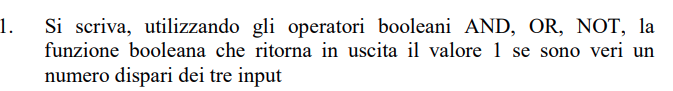
\includegraphics[width=1\linewidth]{es1_pag10_AlgebraDiBoole}
	%\caption{}
	\label{fig:es1pag10algebradiboole}
\end{figure}

\begin{tabular}{|c|c|c||c||c|}
	\hline
	A & B & C & f(a,b,c) & \\
	\hline
	0 & 0 & 0 & 0 & \\
	\hline
	%\rowcolor{BrickRed}
	\tikzmark{starta}0 & 0 & 1 & 1 \tikzmark{enda}& $\bar{\text{A}}\overline{\text{B}}\text{C}$  \\
	\hline
	\tikzmark{startb}0 & 1 & 0 & 1 \tikzmark{endb}& $\overline{\text{A}}\text{B}\overline{\text{C}}$ \\
	\hline
	0 & 1 & 1 & 0 & \\
	\hline
	\tikzmark{startc}1 & 0 & 0 & 1 \tikzmark{endc}& $\text{A}\overline{\text{B}}\overline{\text{C}}$ \\
	\hline
	1 & 0 & 1 & 0 & \\
	\hline
	1 & 1 & 0 & 0 & \\
	\hline
	\tikzmark{startd}1 & 1 & 1 & 1 \tikzmark{endd}& \text{ABC} \\
	\hline  
\end{tabular}

%\markcells{20mm}{1em}
% 	{\circled{\textbf{$M_J=1$}}}& $\textbf{$M_J=2$}$  \\ 
%\begin{comment}
\begin{tikzpicture}[remember picture,overlay]
\foreach \Val in {a, b, c, d}
{
\draw[rounded corners,red,thick]
([shift={(-0.5\tabcolsep,-0.5ex)}]pic cs:start\Val) 
rectangle 
([shift={(0.5\tabcolsep,2ex)}]pic cs:end\Val);
}
\end{tikzpicture}
%\end{comment}

% BUG: PER VIA DEI TIKZMARKS, DA FIXARE.
% BUG FIXATO: Non dare lo stesso nome alle cose in tikzmark e nella tikzpicture.

\begin{comment}

\begin{tikzpicture}[overlay]
	\draw[red, line width=1.5pt] (1,0.3) ellipse (1cm and 0.2cm);
	\draw[blue] (0.35,0.5) ellipse (0.2cm and 0.5cm);
\end{tikzpicture} 

\end{comment}

$ f(\text{A,B,C}) = \bar{\text{A}}\overline{\text{B}}\text{C} + \overline{\text{A}}\text{B}\overline{\text{C}} + \text{A}\overline{\text{B}}\overline{\text{C}} + \text{ABC}  \hspace{0.5cm}\textrm{\color{red} SOLUZIONE}$ \\

\textsf{{\small Il \textbf{+} è considerato un \textbf{OR}. La \textbf{moltiplicazione} è considerata un \textbf{AND}. }} \\

% --- ESERCIZIO 2 ALGEBRA DI BOOLE ---

\begin{figure}[ht]
	%\centering
	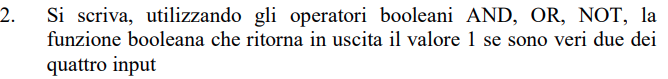
\includegraphics[width=1\linewidth]{es2_pag10_AlgebraDiBoole}
	%\caption{}
	\label{fig:es2pag10algebradiboole}
\end{figure}

\begin{tabular}{|c|c|c|c||c||c|}
	\hline
	A & B & C & D & F & \\
	\hline
	0 & 0 & 0 & 0 & 0 & \\
	\hline
	0 & 0 & 0 & 1 & 0 & \\
	\hline
	0 & 0 & 1 & 0 & 0 & \\
	\hline
	\tikzmark{starte}0 & 0 & 1 & 1 & 1 \tikzmark{ende}& $ \bar{\text{A}}\overline{\text{B}}\text{C}\text{D} $\\
	\hline
	0 & 1 & 0 & 0 & 0 & \\
	\hline
	\tikzmark{startf}0 & 1 & 0 & 1 & 1 \tikzmark{endf}& $ \overline{\text{A}}\text{B}\overline{\text{C}}\text{D} $\\
	\hline
	\tikzmark{startg}0 & 1 & 1 & 0 & 1 \tikzmark{endg}& $ \overline{\text{A}}\text{B}\text{C}\overline{\text{D}} $\\
	\hline
	0 & 1 & 1 & 1 & 0 & \\
	\hline
	1 & 0 & 0 & 0 & 0 & \\
	\hline
	\tikzmark{starth}1 & 0 & 0 & 1 & 1 \tikzmark{endh}& $ \text{A}\bar{\text{B}}\bar{\text{C}}\text{D} $ \\
	\hline
	\tikzmark{starti}1 & 0 & 1 & 0 & 1 \tikzmark{endi}& $ \text{A}\overline{\text{B}}\text{C}\overline{\text{D}} $\\
	\hline
	1 & 0 & 1 & 1 & 0 & \\
	\hline
	\tikzmark{startl}1 & 1 & 0 & 0 & 1 \tikzmark{endl}& $ \text{AB}\bar{\text{C}}\bar{\text{D}} $ \\
	\hline
	1 & 1 & 0 & 1 & 0 & \\
	\hline
	1 & 1 & 1 & 0 & 0 & \\
	\hline
	1 & 1 & 1 & 1 & 0 & \\
	\hline
\end{tabular}
%\begin{comment}
\begin{tikzpicture}[remember picture,overlay]
	\foreach \Val in {e, f, g, h, i, l}
	{
		\draw[rounded corners,red,thick]
		([shift={(-0.5\tabcolsep,-0.5ex)}]pic cs:start\Val) 
		rectangle 
		([shift={(0.5\tabcolsep,2ex)}]pic cs:end\Val);
	}
\end{tikzpicture}
%\end{comment}
\enlargethispage{90pt}
$ f(\text{A,B,C,D}) = \bar{\text{A}}\overline{\text{B}}\text{C}\text{D} + \overline{\text{A}}\text{B}\overline{\text{C}}\text{D} + \overline{\text{A}}\text{B}\text{C}\overline{\text{D}} + \text{A}\bar{\text{B}}\bar{\text{C}}\text{D} + \text{A}\overline{\text{B}}\text{C}\overline{\text{D}} + \text{AB}\bar{\text{C}}\bar{\text{D}} \hspace{0.5cm}\textrm{\color{red} SOLUZIONE}$ \\

% --- ESERCIZIO 3 ALGEBRA DI BOOLE ---

\newpage

\begin{figure}[ht]
	%\centering
	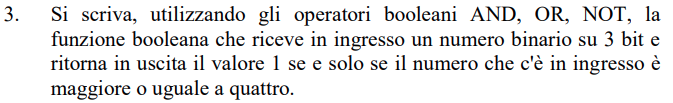
\includegraphics[width=1\linewidth]{es3_pag10_AlgebraDiBoole}
	%\caption{}
	\label{fig:es3pag10algebradiboole}
\end{figure}

\textsf{{\small 3 variabili (A,B,C) e quindi 8 combinazioni}} \\
\begin{itemize}
	\item \textsf{{\small Nella prima a destra (la C) ripetizioni 0 1 (in verticale)}} \\
	\item \textsf{{\small Nella centrale (la B) ripetizione: 0 0 1 1 (in verticale)}} \\
	\item \textsf{{\small In quella a sinistra (la A) ripetizioni 0 0 0 0 1 1 1 1}} \\
\end{itemize}

\begin{tabular}{|c|c|c||c||c|}
	\hline
	A & B & C & f(a,b,c) & \\
	\hline
	0 & 0 & 0 & 0 & \\
	\hline
	0 & 0 & 1 & 0 & \\
	\hline
	0 & 1 & 0 & 0 & \\
	\hline
	0 & 1 & 1 & 0 & \\
	\hline
	\tikzmark{startup}1 & 0 & 0 & 1 \tikzmark{endup}& \text{A}$ \bar{\text{B}}\bar{\text{C}} $\\
	\hline
	\tikzmark{startup2}1 & 0 & 1 & 1 \tikzmark{endup2}& \text{A}$ \overline{\text{B}} $ \text{C}\\
	\hline
	\tikzmark{startdown}1 & 1 & 0 & 1 \tikzmark{enddown}& \text{AB}$ \overline{\text{C}} $\\
	\hline
	\tikzmark{startdown2}1 & 1 & 1 & 1 \tikzmark{enddown2}& \text{ABC} \\
	\hline  
\end{tabular}

%\begin{comment}
\begin{tikzpicture}[remember picture,overlay]
	\foreach \Val in {up, up2, down, down2}
	{
		\draw[rounded corners,red,thick]
		([shift={(-0.5\tabcolsep,-0.5ex)}]pic cs:start\Val) 
		rectangle 
		([shift={(0.5\tabcolsep,2ex)}]pic cs:end\Val);
	}
\end{tikzpicture}
%\end{comment}

\begin{tikzpicture}[overlay]
	%\draw[red, line width=1.5pt] (1,0.3) ellipse (1cm and 0.2cm);
	%\draw[blue, line width=.9pt] (0.35,1.6) ellipse (0.2cm and 1.2cm);
	\draw[blue, line width=.9pt] (0.35,2.7) ellipse (0.2cm and 2.2cm);
	\draw[blue, line width=.9pt] (3.1,2.7) ellipse (0.2cm and 2.2cm);
\end{tikzpicture}

$ f(\text{A,B,C}) = \text{A}\bar{\text{B}}\bar{\text{C}} + \text{A}\overline{\text{B}} \text{C} + \text{AB} \overline{\text{C}} + \text{ABC} \hspace{0.5cm} \textrm{\color{red} SOLUZIONE}$ \\

\textsf{{\small La soluzione può anche essere scritta: }} \\

$ f(\text{A,B,C}) = \text{A} $ \\

\textsf{{\small La colonna A è uguale alla colonna di F (non solo quei quattro 1, ma tutta la colonna dall'inizio, zeri compresi), se dovessi solo restituire A è come se restituissi F.}} \\

% --- ESERCIZIO 4 ALGEBRA DI BOOLE ---

\pagebreak

\begin{figure}[ht]
	%\centering
	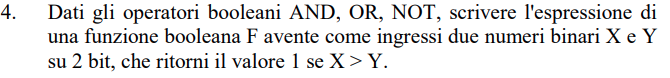
\includegraphics[width=1\linewidth]{es4_pag10_AlgebraDiBoole}
	%\caption{}
	\label{fig:es4pag10algebradiboole}
\end{figure}
%\enlargethispage{320pt}
\begin{tabular}{|c|c|c|c||c||c|c|c|}
	\hline
	$\color{blue}\mathbf{x_1}$ & $\color{blue}\mathbf{x_0}$ & $\color{green}\mathbf{y_1}$ & $\mathbf{\color{green}y_0}$ & $f(x,y)$ & $ \mathbf{\color{blue}x_1 x_0}$& $ \mathbf{\color{green} y_1 y_0} $ &\\
	\hline
	0 & 0 & 0 & 0 & \color{red}0 & \color{blue}0 & \color{green}0 &\\
	\hline
	0 & 0 & 0 & 1 & \color{red}0 & \color{blue}0 & \color{green}1 &\\
	\hline
	0 & 0 & 1 & 0 & \color{red}0 & \color{blue}0 & \color{green}2 &\\
	\hline
	0 & 0 & 1 & 1 & \color{red}0 & \color{blue}0 & \color{green}3 &\\
	\hline
	\tikzmark{startm}0 & 1 & 0 & 0 & \color{red}1\tikzmark{endm} & \color{blue}1 & \color{green}0& $ \mathbf{\overline{x_1}x_0\overline{y_1}\bar{y_0}} $\\
	\hline
	0 & 1 & 0 & 1 & \color{red}0 & \color{blue}1 & \color{green} 1 &\\
	\hline
	0 & 1 & 1 & 0 & \color{red}0 & \color{blue}1 & \color{green} 2 &\\
	\hline
	0 & 1 & 1 & 1 & \color{red}0 & \color{blue}1 & \color{green}3 &\\
	\hline
	\tikzmark{startn}1 & 0 & 0 & 0 & \color{red}1\tikzmark{endn} & \color{blue}2 & \color{green}0 & $ \mathbf{x_1\overline{x_0}\bar{y_1}\overline{y_0}} $\\
	\hline
	\tikzmark{starto}1 & 0 & 0 & 1 & \color{red}1\tikzmark{endo} & \color{blue}2 & \color{green}1 & $ \mathbf{x_1 x_0 \bar{y_1}\overline{y_0}} $ \\
	\hline
	1 & 0 & 1 & 0 & \color{red}0 & \color{blue}2 & \color{green}2 &\\
	\hline
	1 & 0 & 1 & 1 & \color{red}0 & \color{blue}2 & \color{green}3 &\\
	\hline
	\tikzmark{startp}1 & 1 & 0 & 0 & \color{red}1\tikzmark{endp} & \color{blue}3 & \color{green}0 & $ \mathbf{x_1 x_0 \bar{y_1} \overline{y_0}} $\\
	\hline
	\tikzmark{startq}1 & 1 & 0 & 1 & \color{red}1\tikzmark{endq} & \color{blue}3 & \color{green}1 & $ \mathbf{x_1 x_0 \overline{y_1} y_0} $\\
	\hline
	\tikzmark{startr}1 & 1 & 1 & 0 & \color{red}1\tikzmark{endr} & \color{blue}3 & \color{green}2 & $ \mathbf{x_1 x_0 y_1 \overline{y_0}} $\\
	\hline
	1 & 1 & 1 & 1 & \color{red}0 & \color{blue}3 & \color{green}3 &\\
	\hline
\end{tabular}
%\begin{comment}
\begin{tikzpicture}[remember picture,overlay]
\foreach \Val in {m, n, o, p, q, r}
{
\draw[rounded corners,blue,thick]
([shift={(-0.5\tabcolsep,-0.5ex)}]pic cs:start\Val) 
rectangle 
([shift={(0.5\tabcolsep,2ex)}]pic cs:end\Val);
}
\end{tikzpicture}
%\end{comment}

$ f(x,y) = \mathbf{\overline{x_1}x_0\overline{y_1}\bar{y_0}} + \mathbf{x_1\overline{x_0}\bar{y_1}\overline{y_0}} + \mathbf{x_1 x_0 \bar{y_1}\overline{y_0}} + \mathbf{x_1 x_0 \bar{y_1} \overline{y_0}} + \mathbf{x_1 x_0 \overline{y_1} y_0} + \mathbf{x_1 x_0 y_1 \overline{y_0}}$ \\

\textsf{{\small Le colonne: $ \mathbf{\color{blue} x_1 x_0} \text{ e } \mathbf{\color{green}y_1 y_0 }$ sono in decimale considerando due bit.}} \\

% --- TABELLA PROPRITA' FUNZIONI BOOLEANE ---

\subsection{Tabella delle Proprietà delle Funzioni Booleane}

\begin{figure}[ht]
	\centering
	\includegraphics[width=0.7\linewidth]{tabella_proprietà_funzioni_booleane}
	%\caption{Tabella delle Proprietà delle Funzioni Booleane}
	\label{fig:tabella_proprietà_funzioni_booleane}
\end{figure}

% --- ESERCIZIO 5 ALGEBRA DI BOOLE ---

\newpage

\begin{figure}[ht]
	%\centering
	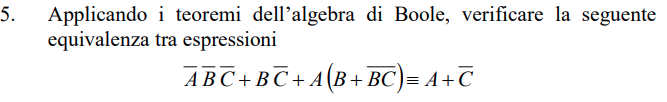
\includegraphics[width=1\linewidth]{es5_pag11_AlgebraDiBoole}
	%\caption{}
	\label{fig:es5pag11algebradiboole}
\end{figure}

\textsf{{\small Cerchiamo di semplificare l'espressione}} \\
 
\begin{equation*}
	\underbrace{\negatoA\negatoBbar\negatoC + \B\negatoC} _{\negatoC(\negatoAbar\negatoB + \B) \hspace{0.3cm}\textrm{\color{red}PROPRIETA' DISTRIBUTIVA}} + 
	\A(\B + \underbrace{\negatoB\negatoC)} 
	_{\A(\B + \negatoB + \negatoC) \hspace{0.3cm}\textrm{\color{red} APPLICHIAMO DE MORGAN}}
\end{equation*}

\begin{equation*}
\negatoC(\underbrace{\negatoAbar\negatoB + \B} _{\negatoC((\negatoA + \B) \cdot (\negatoB + \B)) \textrm{\color{red} \hspace{0.2cm}distr.}}) + \A(\underbrace{\B + \negatoB} _{\A(1 + \negatoC) \hspace{0.2cm}\textrm{\color{red}inverse law}} + \negatoC) 
\end{equation*}

\begin{equation*}
	\C((\negatoA + \B) \cdot (\underbrace{\negatoB + \B} _{\inverse}) ) + \A(\underbrace{1 + \negatoC} _{\nulllaw})
\end{equation*}

\begin{equation*}
	\negatoC(\underbrace{(\negatoA + \B) \cdot 1} _{\identity}) + \underbrace{\A \cdot 1} _{\identity}
\end{equation*}

\begin{equation*}
	\underbrace{\negatoC(\negatoA + \B)} _{\distr} + \A
\end{equation*}

\begin{equation*}
	\underbrace{\negatoC\negatoAbar + \negatoC\B + \A} _{\distr}
\end{equation*}

\begin{equation*}
	(\A + \negatoC)(\underbrace{\A + \negatoA} _{\inverse}) + \negatoC\B
\end{equation*}

\begin{equation*}
	\underbrace{(\A + \negatoC) \cdot 1} _{\identity} + \negatoC\B
\end{equation*}

\begin{equation*}
	(\A + \negatoC) + \negatoC\B
\end{equation*}

\begin{equation*}
\A + \underbrace{\negatoC + \negatoC\B} _{\absorption}
\end{equation*}

\begin{equation*}
	\A + \negatoC
\end{equation*}

% --- ESERCIZIO 6 ---

\pagebreak

\begin{figure}[ht]
	%\centering
	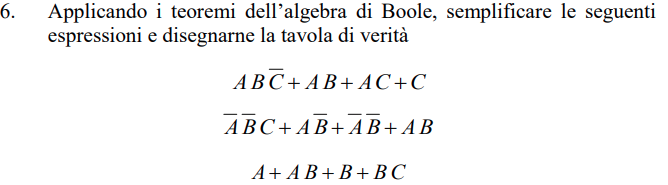
\includegraphics[width=1\linewidth]{es6_pag11_AlgebraDiBoole}
	%\caption{}
	\label{fig:es6pag11algebradiboole}
\end{figure}

\centering
 $\underbrace{\A\B\negatoC + \A\B} _{\absorption} + \underbrace{\A\C + \C} _{\absorption}  $\\
	 $\A\B + \C $ \\
\flushleft

\begin{tabular}{|c|c|c|c||c||c|c|c|}
	\hline
	A & B & C & $\overset{x}{\A\B}$ & $\overset{y}{\A\C}$ & $\overset{z}{AB\negatoC}$ & $ z + x + y + c $ & $x + c$\\
	\hline
	0 & 0 & 0 & 0 & 0 & 0 & 0 & 0\\
	\hline
	0 & 0 & 1 & 0 & 0 & 0 & 1 & 1\\
	\hline
	0 & 1 & 0 & 0 & 0 & 0 & 0 & 0\\
	\hline
	0 & 1 & 1 & 0 & 0 & 0 & 1 & 1\\
	\hline
	1 & 0 & 0 & 0 & 0 & 0 & 0 & 0\\
	\hline
	1 & 0 & 1 & 0 & 1 & 0 & 1 & 1\\
	\hline
	1 & 1 & 0 & 1 & 0 & 1 & 1 & 1\\
	\hline
	1 & 1 & 1 & 1 & 1 & 0 & 1 & 1\\
	\hline
\end{tabular}

\begin{tikzpicture}[overlay]
	%\draw[red, line width=1.5pt] (1,0.3) ellipse (1cm and 0.2cm);
	\draw[red, line width=.9pt] (6.87,2.1) ellipse (0.2cm and 2.2cm);
	\draw[red, line width=.9pt] (8.75,2.1) ellipse (0.2cm and 2.2cm);
	%\draw[blue, line width=.9pt] (3.1,2.7) ellipse (0.2cm and 2.2cm);
\end{tikzpicture}

\textsf{{\small Le due colonne cerchiate in \textcolor{red}{rosso} sono equivalenti.}} \\

\textrm{\color{red} ES.6 - N.2} \\

\centering
$ \underbrace{\negatoA\negatoBbar} _{\absorption} \C + \A\negatoB + \underbrace{\negatoA\negatoBbar} _{\absorption} + \A\B $ \\

$ \negatoA\negatoBbar + \underbrace{\A\negatoB + \A\B} _{\distr} $ \\

$ \negatoA\negatoBbar + \A(\underbrace{\negatoB + \B} _{\inverse}) $ \\

$ \negatoA\negatoBbar + \underbrace{\A \cdot 1} _{\identity} $ \\

$ \underbrace{\negatoA\negatoBbar + \negatoA} _{\distr} $ \\

$ \underbrace{(\A + \negatoA)} _{\inverse}(\A + \negatoB) $ \\

$ \underbrace{1 \cdot(\A + \negatoB)} _{\identity} $ \\

$ \color{red}\boxed{\normalcolor\A + \negatoB} $ \\

\enlargethispage{30pt}
\textsf{{\small Ora non più semplificabile.}} \\

\centering

\pagebreak

\begin{tabular}{|c|c|c|c||c||c|c|c|c|}
	\hline
	A & B & C & $\overset{x}{\negatoA\negatoBbar}$ & $\overset{y}{X\C}$ & $\overset{z}{A\negatoB}$ & $ \overset{t}{\A\B} $ &$ y + z + x + t $ & $\A + \negatoB$\\
	\hline
	0 & 0 & 0 & 1 & 0 & 0 & 0 & 1 & 1\\
	\hline
	0 & 0 & 1 & 1 & 1 & 0 & 0 & 1 & 1\\
	\hline
	0 & 1 & 0 & 0 & 0 & 0 & 0 & 0 & 0\\
	\hline
	0 & 1 & 1 & 0 & 0 & 0 & 0 & 0 & 0\\
	\hline
	1 & 0 & 0 & 0 & 0 & 1 & 0 & 1 & 1\\
	\hline
	1 & 0 & 1 & 0 & 1 & 1 & 0 & 1 & 1\\
	\hline
	1 & 1 & 0 & 0 & 0 & 0 & 1 & 1 & 1\\
	\hline
	1 & 1 & 1 & 0 & 0 & 0 & 1 & 1 & 1\\
	\hline
\end{tabular}

\begin{tikzpicture}[overlay]
	%\draw[red, line width=1.5pt] (1,0.3) ellipse (1cm and 0.2cm);
	\draw[red, line width=.9pt] (2.45,2.1) ellipse (0.2cm and 2.2cm);
	\draw[red, line width=.9pt] (4.42,2.1) ellipse (0.2cm and 2.2cm);
	%\draw[blue, line width=.9pt] (3.1,2.7) ellipse (0.2cm and 2.2cm);
\end{tikzpicture}

\textsf{{\small Le due colonne cerchiate in \textcolor{red}{rosso} sono equivalenti.}} \\

\flushleft

% --- ESERCIZIO 7 ALGEBRA DI BOOLE ---

\begin{figure}[ht]
	%\centering
	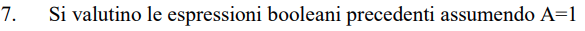
\includegraphics[width=1\linewidth]{es7_pag11_AlgebraDiBoole}
	%\caption{}
	\label{fig:es7pag11algebradiboole}
\end{figure}

\pagebreak

% --- ESERCIZIO 8 ALGEBRA DI BOOLE ---

\begin{figure}[ht]
	%\centering
	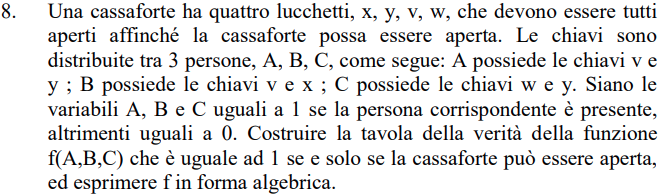
\includegraphics[width=1\linewidth]{es8_pag11_AlgebraDiBoole}
	%\caption{}
	\label{fig:es8pag11algebradiboole}
\end{figure}

\centering

\begin{tabular}{|c|c|c||c||c|}
	\hline
	A & B & C & $f$ & \\
	\hline
	0 & 0 & 0 & 0 & \\
	\hline
	0 & 0 & 1 & 0 & \\
	\hline
	0 & 1 & 0 & 0 & \\
	\hline
	\tikzmark{starts}0 & 1 & 1 & 1 \tikzmark{ends}& $ \negatoA\B\C $\\
	\hline
	1 & 0 & 0 & 0 & \\
	\hline
	1 & 0 & 1 & 0 & \\
	\hline
	1 & 1 & 0 & 0 & \\
	\hline
	\tikzmark{startt}1 & 1 & 1 & 1 \tikzmark{endt}& \A\B\C \\
	\hline  
\end{tabular}

\begin{tikzpicture}[remember picture,overlay]
	\foreach \Val in {s, t}
	{
		\draw[rounded corners,red,thick]
		([shift={(-0.5\tabcolsep,-0.5ex)}]pic cs:start\Val) 
		rectangle 
		([shift={(0.5\tabcolsep,2ex)}]pic cs:end\Val);
	}
\end{tikzpicture}

\centering

$ f(\A, \B, \C) = \underbrace{\negatoA\B\C + \A\B\C} _{\distr} $ \\

$ \B\C\underbrace{(\negatoA + \A)} _{\inverse} $ \\

$ \underbrace{\B\C \cdot 1} _{\identity} $ \\

$ \color{red}\boxed{\normalcolor\B\C} \hspace{0.3cm}\textrm{\color{red} SOLUZIONE}$ \\

% --- NOT OR AND LOGIC GATES ---

\subsection{NOT - OR - AND | LOGIC GATES}

\begin{figure}[ht]
	%\centering
	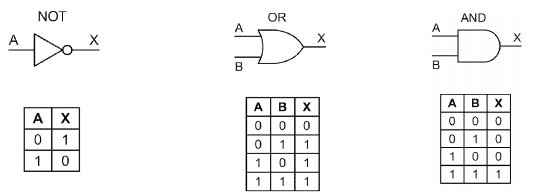
\includegraphics[width=.8\linewidth]{not_or_and_logic_gates}
	%\caption{}
	\label{fig:not_or_and_logic_gates}
\end{figure}

% --- ESERCIZIO 9 ALGEBRA DI BOOLE ---

\newpage

\begin{figure}[ht]
	%\centering
	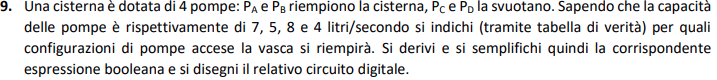
\includegraphics[width=1\linewidth]{es9_esBoole}
	%\caption{}
	\label{fig:es9esBoole}
\end{figure}

%\enlargethispage{120pt}

\begin{tabular}{|c|c|c|c||c||c|}
	\hline
	A & B & C & D & $f$ & \\
	\hline
	0 & 0 & 0 & 0 & 0 & \\
	\hline
	0 & 0 & 0 & 1 & 0 & \\
	\hline
	0 & 0 & 1 & 0 & 0 & \\
	\hline
	0 & 0 & 1 & 1 & 0 & \\
	\hline
	\tikzmark{startu}0 & 1 & 0 & 0 & 1 \tikzmark{endu}& $ \negatoA\B\negatoC\negatoDbar $\\
	\hline
	\tikzmark{startv}0 & 1 & 0 & 1 & 1 \tikzmark{endv}& $ \negatoA\B\negatoC\D $\\
	\hline
	0 & 1 & 1 & 0 & 0 & \\
	\hline
	0 & 1 & 1 & 1 & 0 & \\
	\hline
	\tikzmark{startz}1 & 0 & 0 & 0 & 1 \tikzmark{endz}& $ \A\negatoB\negatoCbar\negatoD $\\
	\hline
	\tikzmark{startw}1 & 0 & 0 & 1 & 1 \tikzmark{endw}& $ \A\negatoB\negatoCbar\D $\\
	\hline
	1 & 0 & 1 & 0 & 0 & \\
	\hline
	1 & 0 & 1 & 1 & 0 & \\
	\hline
	\tikzmark{startj}1 & 1 & 0 & 0 & 1 \tikzmark{endj}& $ \A\B\negatoC\negatoDbar $\\
	\hline
	\tikzmark{starty}1 & 1 & 0 & 1 & 1 \tikzmark{endy}& $ \A\B\negatoC\D $\\
	\hline
	\tikzmark{startx}1 & 1 & 1 & 0 & 1 \tikzmark{endx}& $ \A\B\C\negatoD $\\
	\hline
	1 & 1 & 1 & 1 & 0 & \\
	\hline
\end{tabular}

\begin{tikzpicture}[remember picture,overlay]
	\foreach \Val in {u, v, z, w, j, y, x}
	{
		\draw[rounded corners,red,thick]
		([shift={(-0.5\tabcolsep,-0.5ex)}]pic cs:start\Val) 
		rectangle 
		([shift={(0.5\tabcolsep,2ex)}]pic cs:end\Val);
	}
\end{tikzpicture}

	
$ f(\A, \B, \C, \D) = \negatoA\B\negatoC\negatoDbar + \negatoA\B\negatoC\D + \A\negatoB\negatoCbar\negatoD + \A\negatoB\negatoCbar\D + \A\B\negatoC\negatoDbar + \A\B\negatoC\D + \A\B\C\negatoD $ \break

$ \underbrace{\negatoA\B\negatoC\negatoDbar + \negatoA\B\negatoC\D} _{} + \underbrace{\A\negatoB\negatoCbar\negatoD + \A\negatoB\negatoCbar\D} _{} + \underbrace{\A\B\negatoC\negatoDbar + \A\B\negatoC\D} _{} + \A\B\C\negatoD + \negatoA\B\negatoC(\underbrace{\negatoD + \D} _{\inverse}) + \A\negatoBbar\negatoC(\underbrace{\negatoD + \D} _{\inverse}) + \A\B\negatoC(\underbrace{\negatoD + \D} _{\inverse}) $ \\

$ \Rightarrow \negatoA\B\negatoC + \A\negatoBbar\negatoC + \underbrace{\A\B\negatoC + \A\B\C\negatoD} _{} + \A\B(\underbrace{\negatoC + \C\negatoD} _{\negatoC + \negatoD})$ \\

$ \underbrace{\negatoA\B\negatoC} _{} + \A\negatoBbar\negatoC + \underbrace{\A\B\negatoC} _{} + \A\B\negatoD$ \\

$ \B\negatoC(\underbrace{\negatoA + \A} _{1\inverse}) $ \\

$ \underbrace{\B\negatoC + \A\negatoBbar\negatoC} _{} + \A\B\negatoD + \negatoC(\underbrace{\A + \A\negatoB} _{\B + \A})$ \\

$ \A\negatoC + \underbrace{\B\negatoC + \A\B\negatoD} _{\B(\negatoC + \A\negatoD)} $ \\

$ \color{red}\boxed{\normalcolor\A\negatoC + \B(\negatoC + \A\negatoD)} \hspace{0.3cm}\SOLUZIONE$ \\

\begin{comment}
\begin{circuitikz} \draw
	(0,2) node[and port] (myand1) {}
	(0,0) node[and port] (myand2) {}
	(2,1) node[xnor port] (myxnor) {}
	(myand1.out) -- (myxnor.in 1)
	(myand2.out) -- (myxnor.in 2);
\end{circuitikz}
\end{comment}

\begin{comment}
\begin{tikzpicture}[label distance=2mm]
	
	\node (x3) at (0,0) {\A};
	\node (x2) at (1,0) {\B};
	\node (x1) at (2,0) {\C};
	\node (x0) at (3,0) {\D};
	
	\node (x4) at (0.5, -0.3) {$ \negatoA $};
	\node (x5) at (1.5, -0.3) {$ \negatoB $};
	\node (x6) at (2.5, -0.3) {$ \negatoC $};
	\node (x7) at (3.5, -0.3) {$ \negatoD $};
	
	\node[not gate US, draw, rotate=-90] at ($(x3)+(0.5,-1)$) (Not3) {};
	\node[not gate US, draw, rotate=-90] at ($(x2)+(0.5,-1)$) (Not2) {};
	\node[not gate US, draw, rotate=-90] at ($(x1)+(0.5,-1)$) (Not1) {};
	\node[not gate US, draw, rotate=-90] at ($(x0)+(0.5,-1)$) (Not0) {};
	
	\node[or gate US, draw, logic gate inputs=nnn] at ($(x0)+(2,-2)$) (Or1) {};
	\node[or gate US, draw, logic gate inputs=nnnn] at ($(Or1)+(0,-1)$) (Or2) {};
	\node[or gate US, draw, logic gate inputs=nnn] at ($(Or2)+(0,-1)$) (Or3) {};
	\node[xor gate US, draw, logic gate inputs=nn] at ($(Or3)+(0,-1)$) (Xor1) {};
	\node[and gate US, draw, logic gate inputs=nn, anchor=input 1] at ($(Or3.output)+(1,0)$) (And1) {};
	\node[nor gate US, draw, logic gate inputs=nn, anchor=input 1] at ($(Or2.output -| And1.output)+(1,0)$) (Nor1) {};
	\node[and gate US, draw, logic gate inputs=nn, anchor=input 1] at ($(Or1.output -| Nor1.output)+(1,0)$) (And2) {};
	
	\foreach \i in {2,1,0}
	{
		\path (x\i) -- coordinate (punt\i) (x\i |- Not\i.input);
		\draw (punt\i) node[branch] {} -| (Not\i.input);
	}
	\draw (x3) |- (Or2.input 1);
	\draw (x3 |- Or1.input 1) node[branch] {} -- (Or1.input 1);
	\draw (x2) |- (Xor1.input 1);
	\draw (x2 |- Or3.input 1) node[branch] {} -- (Or3.input 1);
	\draw (Not2.output) |- (Or2.input 2);
	\draw (x1) |- (Or3.input 2);
	\draw (x1 |- Or1.input 2) node[branch] {} -- (Or1.input 2);
	\draw (Not1.output) |- (Xor1.input 2);
	\draw (Not1.output |- Or2.input 3) node[branch] {} -- (Or2.input 3);
	\draw (x0) |- (Or2.input 4);
	\draw (Not0.output) |- (Or3.input 3);
	\draw (Not0.output |- Or1.input 3) node[branch] {} -- (Or1.input 3);
	\draw (Or3.output) -- (And1.input 1);
	\draw (Xor1.output) -- ([xshift=0.5cm]Xor1.output) |- (And1.input 2);
	\draw (Or2.output) -- (Nor1.input 1);
	\draw (And1.output) -- ([xshift=0.5cm]And1.output) |- (Nor1.input 2);
	\draw (Or1.output) -- (And2.input 1);
	\draw (Nor1.output) -- ([xshift=0.5cm]Nor1.output) |- (And2.input 2);
	\draw (And2.output) -- ([xshift=0.5cm]And2.output) node[above] {$f_1$};
\end{tikzpicture}
\end{comment}

\begin{tikzpicture}[label distance=2mm]
	
	\node (x3) at (0,0) {\A};
	\node (x2) at (1,0) {\B};
	\node (x1) at (2,0) {\C};
	\node (x0) at (3,0) {\D};
	
	\node (x4) at (0.5, -0.3) {$ \negatoA $};
	\node (x5) at (1.5, -0.3) {$ \negatoB $};
	\node (x6) at (2.5, -0.3) {$ \negatoC $};
	\node (x7) at (3.5, -0.3) {$ \negatoD $};
	
	\node[not gate US, draw, rotate=-90] at ($(x3)+(0.5,-1)$) (Not3) {};
	\node[not gate US, draw, rotate=-90] at ($(x2)+(0.5,-1)$) (Not2) {};
	\node[not gate US, draw, rotate=-90] at ($(x1)+(0.5,-1)$) (Not1) {};
	\node[not gate US, draw, rotate=-90] at ($(x0)+(0.5,-1)$) (Not0) {};
	
	%\begin{comment}
	\node[and gate US, draw, logic gate inputs=nn] at ($(x0)+(2,-2)$) (And1) {\text{\tiny AND}};
	\node[and gate US, draw, logic gate inputs=nn] at ($(And1)+(0,-1)$) (And2) {\logicAND};
	%\node[or gate US, draw, logic gate inputs=nn] at ($(And2)+(2,-0.5)$) (Or1) {};
	%\node[and gate US, draw, logic gate inputs=nn] at ($(Or1)+(1,-1)$) (And3) {};
	%\node[or gate US, draw, logic gate inputs=nn] at ($ (And1)+(3, 0)$) (Or2) {};
	\node[or gate US, draw, logic gate inputs=nn, anchor=input 1] at ($(And2.output)+(1,-0.5)$) (Or1) {\logicOR};
	\node[and gate US, draw, logic gate inputs=nn, anchor=input 1] at ($(Or1.output)+(1,-0.5)$) (And3) {\logicAND};
	\node[or gate US, draw, logic gate inputs=nn, anchor=input 1] at ($ (And1.output)+(5, 0) $) (Or2) {\logicOR};
	%\end{comment}
	
	\foreach \i in {3,2,1,0} %aggiungere il 3 se non c'è
	{
		\path (x\i) -- coordinate (punt\i) (x\i |- Not\i.input);
		\draw (punt\i) node[branch] {} -| (Not\i.input);
	}
	%\begin{comment}
	% Allungo le linee A negato e B negato, anche se non vengono utilizzate
	\draw(Not3.output) -- ($(Not3)+(0,-3.35)$);
	\draw(Not2.output) -- ($(Not2)+(0,-3.35)$);
	
	% AND C NEGATO E A
	\draw (x3) |- (And1.input 1); % con questo aggiungo la linea
	\draw (x3 |- And1.input 1) node[branch] {}; %con questo aggiungo il punto
	\draw (Not1.output) |- (And1.input 2);
	\draw (Not1.output |- And1.input 2) node[branch] {};
	
	% AND A E D NEGATO
	\draw (x3) |- (And2.input 1);
	\draw (x3 |- And2.input 1) node[branch] {};
	\draw (Not0.output) |- (And2.input 2);
	\draw (Not0.output |- And2.input 2) node[branch] {};
	
	% OR AND2 OUTPUT E C NEGATO
	\draw (And2.output) -- ([xshift=0.5cm]And2.output) |- (Or1.input 1);
	
	\draw (Not1.output) |- (Or1.input 2);
	\draw (Not1.output |- Or1.input 2) node[branch] {};
	
	% AND Or1.output E B
	\draw (x2) |- (And3.input 2);
	\draw (x2 |- And3.input 2) node[branch] {};
	
	\draw (Or1.output) -- ([xshift=0.5cm]Or1.output) |- (And3.input 1); % questo serve per quello zig zag
	
	% OR And3.output E And1.output
	\draw (And1.output) |- (Or2.input 1);
	\draw (And3.output) -- ([xshift=0.5cm]And3.output) |- (Or2.input 2);
	
	% RIGA FINALE DOPO L'ULTIMO OR (A DESTRA)
	\draw (Or2.output) -- ([xshift=0.5cm]Or2.output); %node[above] {$f_1$};

	%\end{comment}
\end{tikzpicture}

% --- ESERCIZIO 10 ALGEBRA DI BOOLE ---

\begin{figure}[ht]
	%\centering
	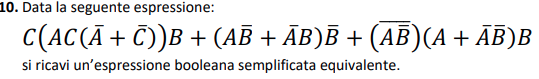
\includegraphics[width=.8\linewidth]{es10_esBoole}
	%\caption{}
	\label{fig:es10esBoole}
\end{figure}

$ \C(\underbrace{\A\C(\negatoA + \negatoC)} _{\underbrace{\A\C\negatoA} _{0} + \underbrace{\A\C\negatoC} _{0}})\B 
+ \underbrace{(\A\negatoB + \negatoA\B)\negatoB} _{\underbrace{\A\negatoBbar\negatoB} _{\A\negatoB} + \underbrace{\negatoA\B\negatoB} _{0}}
+ \underbrace{(\negatoA\overline{\negatoBbar})} _{\negatoA + \B}
+(\underbrace{\A + \negatoA\negatoBbar} _{\A + \negatoB})\B$ \\

$ \Rightarrow 0 \hspace{0.2cm}\text{(Se fossero stati in AND avrebbe azzerato tutto)} + \A\negatoB + 0 + (\negatoA + \B)\underbrace{(\A + \negatoB)\B} _{\A\B + \underbrace{\negatoB\B} _{0}} $ \\

$ \A\negatoB + \underbrace{(\negatoA + \B)\A\B} _{\underbrace{\negatoA\A\B} _{0}
+ \underbrace{\B\A\B} _{\A\B}} $ \\

$ \underbrace{\A\negatoB + \A\B} _{\A(\underbrace{\negatoB + \B} _{1})} $ \\

$ \color{red}\boxed{\normalcolor\A} \hspace{0.3cm}\SOLUZIONE$ \\

% --- ESERCIZIO 11 ALGEBRA DI BOOLE ---

\enlargethispage{18pt}
\begin{figure}[ht]
	%\centering
	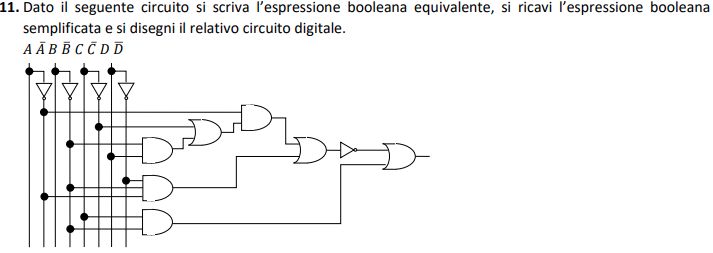
\includegraphics[width=1\linewidth]{es11_esBoole}
	%\caption{}
	\label{fig:es11esBoole}
\end{figure}

$ (\overline{(\underbrace{\negatoB\D + \negatoC)\negatoA} _{\negatoA\negatoBbar\D + \negatoA\negatoCbar} 
	+ \negatoA\negatoBbar\negatoD}) + \negatoB\C$ \\

$ \overline{\negatoA\negatoCbar + \underbrace{\negatoA\negatoBbar\D + \negatoA\negatoBbar\negatoD} _{\negatoA\negatoBbar(\underbrace{\D + \negatoD} _{1})}} + \B\C $ \\

$ \overline{\underbrace{\negatoA\negatoCbar + \negatoA\negatoBbar} _{\demorgan}} + \B\C $ \\

$ \underbrace{(\A + \C)(\A + \B)} _{\A + \B\C} + \B\C $ \\

$ \A + \underbrace{\B\C + \negatoB\C} _{\C(\underbrace{\B + \negatoB} _{1})} $ \\

$ \color{red}\boxed{\normalcolor \A + \C} \hspace{0.3cm}\SOLUZIONE $ \\

\begin{tikzpicture}[label distance=2mm]
	
	\node (x3) at (0,0) {\A};
	\node (x2) at (1,0) {\B};
	\node (x1) at (2,0) {\C};
	\node (x0) at (3,0) {\D};
	
	\node (x4) at (0.5, -0.3) {$ \negatoA $};
	\node (x5) at (1.5, -0.3) {$ \negatoB $};
	\node (x6) at (2.5, -0.3) {$ \negatoC $};
	\node (x7) at (3.5, -0.3) {$ \negatoD $};
	
	\node[not gate US, draw, rotate=-90] at ($(x3)+(0.5,-1)$) (Not3) {};
	\node[not gate US, draw, rotate=-90] at ($(x2)+(0.5,-1)$) (Not2) {};
	\node[not gate US, draw, rotate=-90] at ($(x1)+(0.5,-1)$) (Not1) {};
	\node[not gate US, draw, rotate=-90] at ($(x0)+(0.5,-1)$) (Not0) {};
	
	%\begin{comment}
	\node[or gate US, draw, logic gate inputs=nn] at ($(x0)+(2,-2)$) (Or1) {\text{\logicOR}};
	%\end{comment}
	
	\foreach \i in {3,2,1,0} %aggiungere il 3 se non c'è
	{
		\path (x\i) -- coordinate (punt\i) (x\i |- Not\i.input);
		\draw (punt\i) node[branch] {} -| (Not\i.input);
	}
	%\begin{comment}
	% Allungo le altre linee che non ho usato e anche quelle che ho usato.
	\draw(Not3.output) -- ($(Not3)+(0,-3.35)$);
	\draw(Not2.output) -- ($(Not2)+(0,-3.35)$);
	\draw(Not1.output) -- ($(Not1)+(0,-3.35)$);
	\draw(Not0.output) -- ($(Not0)+(0,-3.35)$);
	
	\draw(x3) -- ($(x3)+(0,-4.35)$);
	\draw(x2) -- ($(x2)+(0,-4.35)$);
	\draw(x1) -- ($(x1)+(0,-4.35)$);
	\draw(x0) -- ($(x0)+(0,-4.35)$);
	
	% OR TRA A E C
	\draw (x3) |- (Or1.input 1);
	\draw (x3 |- Or1.input 1) node[branch] {};
	
	\draw (x1) |- (Or1.input 2);
	\draw (x1 |- Or1.input 2) node[branch] {};
	
	% RIGA FINALE
	\draw (Or1.output) -- ([xshift=0.5cm]Or1.output); %node[above] {$f_1$};
	
	%\end{comment}
\end{tikzpicture}

% --- ESERCIZIO 12 ALGEBRA DI BOOLE ---

\begin{figure}[ht]
	%\centering
	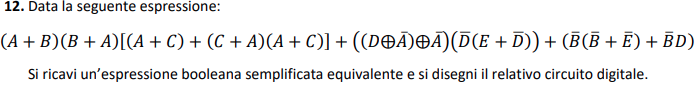
\includegraphics[width=1\linewidth]{es12_esBoole}
	%\caption{}
	\label{fig:es12esBoole}
\end{figure}
%\enlargethispage{60pt}
\begin{equation*}
	\underbrace{(\A + \B)(\B + \A)} _{\A + \B}
	[(\A + \C) + \underbrace{(\C + \A)(\A + \C)} _{\A + \C}] + ((\D\overset{\XOR}{\oplus}\negatoA)\oplus\negatoA)(\underbrace{\negatoD(\E+\negatoD)} _{\negatoD \hspace{0.2cm}\absorption}) + (\underbrace{\negatoB(\negatoB + \negatoE)} _{\negatoB} + \negatoB\D)
\end{equation*}

\begin{equation*}
	(\A + \B)[\underbrace{(\A + \C) + (\A + \C)} _{\A + \C \hspace{0.2cm}\inverse}]
	+ ((\D\oplus\negatoA)\oplus\negatoA)\negatoD + (\underbrace{\negatoB +\negatoB\D} _{\negatoB \hspace{0.2cm}\absorption})
\end{equation*}

\begin{equation*}
	\underbrace{(\A + \B)(\A + \C)} _{\A + \B\C \hspace{0.2cm}\distr} +
	(\underbrace{(\D \oplus \negatoA)\oplus \negatoA} _{\D}) \negatoD + \negatoB
\end{equation*}

\begin{equation*}
	\A + \B\C + \underbrace{\D\negatoD} _{0} + \B
\end{equation*}

\begin{equation*}
	\Rightarrow \A + \underbrace{\B\C + \negatoB} _{\negatoB + \C}
\end{equation*}

\begin{equation*}
	\color{red}\boxed{\normalcolor \A + \negatoB + \C} \hspace{0.3cm}\SOLUZIONE
\end{equation*}


\begin{tikzpicture}[label distance=2mm]
	
	\node (x3) at (0,0) {\A};
	\node (x2) at (1,0) {\B};
	\node (x1) at (2,0) {\C};
	\node (x0) at (3,0) {\D};
	
	\node (x4) at (0.5, -0.3) {$ \negatoA $};
	\node (x5) at (1.5, -0.3) {$ \negatoB $};
	\node (x6) at (2.5, -0.3) {$ \negatoC $};
	\node (x7) at (3.5, -0.3) {$ \negatoD $};
	
	\node[not gate US, draw, rotate=-90] at ($(x3)+(0.5,-1)$) (Not3) {};
	\node[not gate US, draw, rotate=-90] at ($(x2)+(0.5,-1)$) (Not2) {};
	\node[not gate US, draw, rotate=-90] at ($(x1)+(0.5,-1)$) (Not1) {};
	\node[not gate US, draw, rotate=-90] at ($(x0)+(0.5,-1)$) (Not0) {};
	
	%\begin{comment}
	\node[or gate US, draw, logic gate inputs=nnn] at ($(x0)+(2,-2)$) (Or1) {\text{\logicOR}};
	%\end{comment}
	
	\foreach \i in {3,2,1,0} %aggiungere il 3 se non c'è
	{
		\path (x\i) -- coordinate (punt\i) (x\i |- Not\i.input);
		\draw (punt\i) node[branch] {} -| (Not\i.input);
	}
	%\begin{comment}
	% Allungo le altre linee che non ho usato e anche quelle che ho usato.
	\draw(Not3.output) -- ($(Not3)+(0,-3.35)$);
	\draw(Not2.output) -- ($(Not2)+(0,-3.35)$);
	\draw(Not1.output) -- ($(Not1)+(0,-3.35)$);
	\draw(Not0.output) -- ($(Not0)+(0,-3.35)$);
	
	\draw(x3) -- ($(x3)+(0,-4.35)$);
	\draw(x2) -- ($(x2)+(0,-4.35)$);
	\draw(x1) -- ($(x1)+(0,-4.35)$);
	\draw(x0) -- ($(x0)+(0,-4.35)$);
	
	% OR TRA A E B NEGATO E C
	\draw (x3) |- (Or1.input 1);
	\draw (x3 |- Or1.input 1) node[branch] {};
	
	\draw (Not2) |- (Or1.input 2);
	\draw (Not2 |- Or1.input 2) node[branch] {};
	
	\draw (x1) |- (Or1.input 3);
	\draw (x1 |- Or1.input 3) node[branch] {};
	
	% RIGA FINALE
	\draw (Or1.output) -- ([xshift=0.5cm]Or1.output); %node[above] {$f_1$};
	
	%\end{comment}
\end{tikzpicture}

% --- ESERCIZIO 13 ALGEBRA DI BOOLE ---

\begin{figure}[ht]
	%\centering
	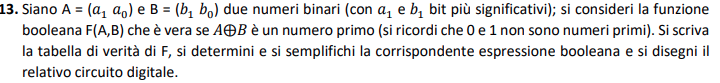
\includegraphics[width=1\linewidth]{es13_esBoole}
	%\caption{}
	\label{fig:es13esBoole}
\end{figure}

\begin{tabular}{|c|c|c|c||c||c||c|}
	\hline
	$a_1$ & $a_0$ & $b_1$ & $b_0$ & $ \A\oplus\B $ & $ F $ &\\
	\hline
	0 & 0 & 0 & 0 & 00 & 0 & \\
	\hline
	0 & 0 & 0 & 1 & 01 & 0 & \\
	\hline
	\tikzmark{startab}0 & 0 & 1 & 0 & 10 & 1 \tikzmark{endab}& $\mathbf{\overline{a_1}\bar{a_0} b_1 \overline{b_0}} $\\
	\hline
	\tikzmark{startbb}0 & 0 & 1 & 1 & 11 & 1 \tikzmark{endbb}& $\mathbf{\overline{a_1}\bar{a_0} b_1 b_0}$\\
	\hline
	0 & 1 & 0 & 0 & 01 & 0 & \\
	\hline
	0 & 1 & 0 & 1 & 00 & 0 & \\
	\hline
	\tikzmark{startcb}0 & 1 & 1 & 0 & 11 & 1 \tikzmark{endcb}& $\mathbf{\overline{a_1}a_0 b_1 \overline{b_0}}$\\
	\hline
	\tikzmark{startdb}0 & 1 & 1 & 1 & 10 & 1 \tikzmark{enddb}& $\mathbf{\overline{a_1}a_0 b_1 b_0}$\\
	\hline
	\tikzmark{starteb}1 & 0 & 0 & 0 & 10 & 1 \tikzmark{endeb}&  $\mathbf{a_1\overline{a_0} \bar{b_1} b_0}$\\
	\hline
	\tikzmark{startfb}1 & 0 & 0 & 1 & 11 & 1 \tikzmark{endfb}& $\mathbf{a_1\overline{a_0} \bar{b_1} b_0}$ \\
	\hline
	1 & 0 & 1 & 0 & 00 & 0 & \\
	\hline
	1 & 0 & 1 & 1 & 01 & 0 & \\
	\hline
	\tikzmark{startgb}1 & 1 & 0 & 0 & 11 & 1 \tikzmark{endgb}& $\mathbf{a_1 a_0 \overline{b_1} \bar{b_0}}$\\
	\hline
	\tikzmark{starthb}1 & 1 & 0 & 1 & 10 & 1 \tikzmark{endhb}& $\mathbf{a_1 a_0 \overline{b_1} b_0}$\\
	\hline
	1 & 1 & 1 & 0 & 01 & 0 & \\
	\hline
	1 & 1 & 1 & 1 & 00 & 0 & \\
	\hline
\end{tabular}

%\begin{comment}
\begin{tikzpicture}[remember picture,overlay]
	\foreach \Val in {ab, bb, cb, db, eb, fb, gb, hb}
	{
		\draw[rounded corners,red,thick]
		([shift={(-0.5\tabcolsep,-0.5ex)}]pic cs:start\Val) 
		rectangle 
		([shift={(0.5\tabcolsep,2ex)}]pic cs:end\Val);
	}
\end{tikzpicture}
%\end{comment}

$ F(a,b,c) = \underbrace{\overline{a_1}\bar{a_0} b_1 \overline{b_0} + \overline{a_1}\bar{a_0} b_1 b_0} 
+ \underbrace{\overline{a_1}a_0 b_1 \overline{b_0} + \overline{a_1}a_0 b_1 b_0} 
+ \underbrace{a_1\overline{a_0} \bar{b_1} b_0 + a_1\overline{a_0} \bar{b_1} b_0}
+ \underbrace{a_1 a_0 \overline{b_1} \bar{b_0} + a_1 a_0 \overline{b_1} b_0}$ \\

$ \color{red}\boxed{\normalcolor \overline{a_1} b_1 + a_1 \overline{b_1}} \hspace{0.3cm}\SOLUZIONE$ \\

$ \color{ForestGreen} a_1 \oplus b_1 $ \\

% --- PRESTAZIONI DEI CALCOLATORI ---

\section{Architetture a Confronto}

\subsection{Prestazioni dei Calcolatori}

\begin{figure}[h]%
	\centering
	\subfloat[\centering Tempo di Esecuzione]{{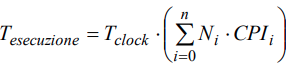
\includegraphics[width=.4\linewidth]{tempo_di_esecuzione}
	\label{fig:tempodiesecuzione} }}%
	\qquad
	\subfloat[\centering Milion Instruction Per Second]{{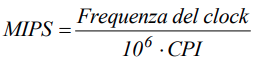
\includegraphics[width=.4\linewidth]{Milion_Instruction_Per_Second} }}%
	%\caption{2 Figures side by side}%
	\label{fig:mips}%
\end{figure}

\begin{figure}[h]%
	\centering
	\subfloat[\centering Prestazione]{{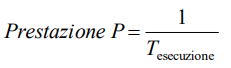
\includegraphics[width=5cm]{prestazione} }}%
	\label{fig:prestazione}
	\qquad
	\subfloat[\centering Legge di Amdhal]{{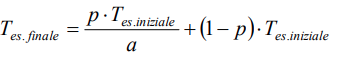
\includegraphics[width=.5\linewidth]{legge_di_amdhal} }}% prima era width=5cm
	%\caption{2 Figures side by side}%
	\label{fig:leggediamdhal}%
\end{figure}


% --- ESERCIZIO 1 MIGLIORAMENTO PRESTAZIONI MEMORIA ---

\newpage 

\begin{figure}[ht]
	%\centering
	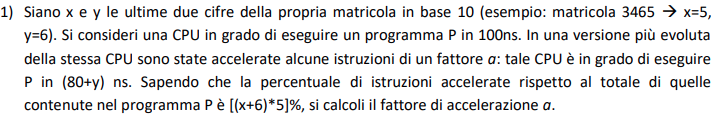
\includegraphics[width=1\linewidth]{es1_MiglioramentoPrestazioneMemoria}
	%\caption{}
	\label{fig:es1MiglioramentoPrestazioneMemoria}
\end{figure}

\textsf{{\small Esempio: matricola 3465 \textrightarrow $x = 5, y = 6$}} \break

\textsf{{\small Matricola (non la mia) = 2602}} \\
$ x = 2 $ \\
$ y = 0 $ \\

$ \text{T}_i \text{ (Tempo iniziale) } = 100 \text{ ns (nanosecondi)} $ \\

$ \text{T}_f \text{ (Tempo finale) } = 80 + y = 80 + 0 = 80 \text{ ns}$ \\

$ P = [(x + 6)\cdot 5]\% \rightarrow [(2 + 6)\cdot 5]\% = 40\% $ \\

$ \alpha = ? $ \\

\textsf{{\large Legge di Amdhal a pag.\pageref{fig:leggediamdhal}}} \\

$ \text{T}_f = \frac{\text{P}\cdot \text{T}_i}{\alpha} + (1 - p) \cdot \text{T}_i $ \\

$ 80 = \frac{0.04 \cdot 100}{\alpha} + 0,6 \cdot 100 $ \\

$ \rightarrow 80 = \frac{40}{\alpha} + 60 \rightarrow 80 - 60 = \frac{40}{\alpha} \rightarrow 20 \cdot \alpha = 40 \rightarrow \color{red}\boxed{\normalcolor\alpha = 2} $ \\

\textrm{\color{red}IL DOPPIO PIU' VELOCE} \\

% --- ESERCIZIO 2 MIGLIORAMENTO PRESTAZIONE MEMORIA ---

\begin{figure}[ht]
	%\centering
	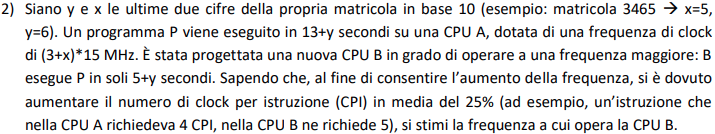
\includegraphics[width=1\linewidth]{es2_MiglioramentoPrestazioneMemoria}
	%\caption{}
	\label{fig:es2MiglioramentoPrestazioneMemoria}
\end{figure}
\enlargethispage{60pt}
\textsf{{\small Matricola = 2602}} $ (x = 2,y = 0) $\\

$ \text{T}_\text{A} = 13 \text{ s (secondi)} $ \\

$ \text{F}_\text{A} = 75 \text{ MHz (MegaHertz)} $ \\

$ \text{T}_\text{B} = 5 \text{ s} $ \\

$ \text{CPI}_\text{B} \text{ (Clock per Instruction)} = 1,25 \cdot \text{CPI}_\text{A} $ \\

$ \text{F}_\text{B} = ? $ \\

\textsf{{\large Prestazioni dei Calcolatori a pag.\pageref{fig:prestazione}}} \\

$ \text{T}_\text{ES} = \text{T}_\text{clock} \cdot \underbrace{\sum_{i = 0}^{n} \text{N}_i \cdot \text{CPI}_i} _{\text{CPI}_\text{TOT}} $ \\

\begin{itemize}
\item\textsf{{\small \textcolor{red}{$\text{T}_\text{clock}$ periodo di clock della macchina} }} \\
\item\textsf{{\small \textcolor{red}{$\text{CPI}_\text{i}$ numero di clock per istruzione di tipo i} numero di clock occorrenti affinchè avvenga l'esecuzione dell'istruzione.}} \\
\item\textsf{{\small \textcolor{red}{$\text{N}_\text{i}$ numero di istruzioni di tipo i} (somme, sottrazioni, salti, ecc..).}} \\
\end{itemize}

\pagebreak

$ \text{T}_\text{ES} \simeq \text{T}_\text{clock} \cdot \text{N}_\text{TOT} \cdot \widetilde{\text{CPI}}  $ \\

\textsf{{\small Quella tilde sopra il CPI significa "Mediamente per ogni istruzione"}} \\

$ \text{T}_\text{clock} = \frac{1}{\text{F}} $ \\

\begin{equation*}
\begin{cases}
13 = \frac{1}{75 \cdot 10^6} \cdot \text{N}_\text{TOT} \cdot\widetilde{\text{CPI}} \\
5 = \frac{1}{\text{F}_\text{B}} \cdot \text{N}_\text{TOT} \cdot \widetilde{\text{CPI}}_\text{B} \\
\end{cases}
\end{equation*}

\textsf{{\small $\text{N}_\text{TOT} $ c'è due volte perchè è lo stesso programma e quindi stesse istruzioni}}  \\

\noindent\begin{minipage}{.5\linewidth}
\begin{equation*}
\begin{cases}
13 \cdot 75 \cdot 10^6 = \text{N}_\text{TOT} \cdot \widetilde{\text{CPI}}_\text{A} \\
5 \cdot \text{F}_\text{B} = \text{N}_\text{TOT} \cdot 1,25 \cdot \widetilde{\text{CPI}}_\text{A} \\
\end{cases}
\end{equation*}
\end{minipage}
\begin{minipage}{.35\linewidth}
	\begin{equation*}
		\begin{cases}
			975 \cdot 10^6 = \text{N}_\text{TOT} \cdot \widetilde{\text{CPI}}_\text{A} \\
		    \text{F}_\text{B} = \frac{1,25 \cdot \text{\color{red}\sout{\normalcolor975}} \cdot 10^6}{\text{\color{red}\sout{\normalcolor5}}} \\
		\end{cases}
	\end{equation*}
\end{minipage}

$ \text{F}_\text{B} = 243,75 \cdot 10^6 \text{ Hz} = 243,75 \text{ Mhz} $ \\

% --- ESERCIZIO 3 MIGLIORAMENTO PRESTAZIONI MEMORIA ---

\begin{figure}[ht]
	%\centering
	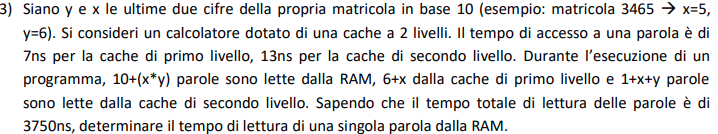
\includegraphics[width=1\linewidth]{es3_MiglioramentoPrestazioneMemoria}
	%\caption{}
	\label{fig:es3MiglioramentoPrestazioneMemoria}
\end{figure}

$ \text{MATR } = 2602 \hspace{0.1cm}(x = 2, y = 0) $ \\

$\text{T}_\text{C1} = 7 \text{ ns} $\\
$\text{T}_\text{C2} = 13 \text{ ns} $\\

\[
\begin{rcases*}
	\text{N}_\text{RAM} = 10 + (x \cdot y) \\
	\text{N}_\text{C1} = 8 \\
	\text{N}_\text{C2} = 3 \\
\end{rcases*} \text{21 ($ \text{N}_\text{TOT}$) PAROLE}
\]

$ \text{T}_\text{TOT} = 3750 \text{ ns} $ \\
$ \text{T}_\text{RAM} = ? $ \\

$ \text{T}_\text{TOT} = (\text{N}_\text{TOT} \cdot \text{T}_\text{C1}) + [(\text{N}_\text{TOT} - \text{N}_\text{C1}) \cdot \text{T}_\text{C2}] + \cdots + [(\text{N}_\text{TOT} - \text{N}_\text{C1} - \text{N}_\text{C2}) \cdot \text{T}_\text{RAM}] $ \\

\textsf{{\small Parole da cercare $(\text{N}_\text{TOT})$ , nella cache L1 $(\text{T}_\text{C1})$ , Parole da cercare meno quelle che ho già trovato nella cache 1 $(\text{N}_\text{TOT} - \text{N}_\text{C1})$}} \\

$ 3750 = 21 \cdot 7 + (21 - 8) \cdot 13 + (21 - 8 - 3) \cdot \text{T}_\text{RAM} $ \\

$ 3750 = 147 + 169 + 10 \cdot \text{T}_\text{RAM} $ \\

$ \frac{3750 - 147 - 169}{10} = \text{T}_\text{RAM} \Rightarrow \text{T}_\text{RAM} \simeq \color{red}\boxed{\normalcolor343,3 \text{ ns}} $ \\

\textsf{{\footnotesize Esercizi non necessariamente realistici.}} \\

% --- ESERCIZIO 4 MIGLIORAMENTO PRESTAZIONI MEMORIA ---

\pagebreak

\begin{figure}[ht]
	%\centering
	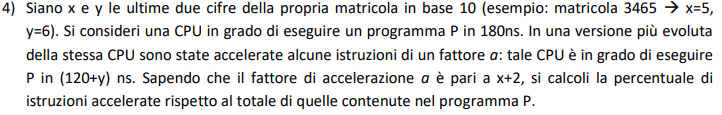
\includegraphics[width=1\linewidth]{es4_MiglioramentoPrestazioneMemoria}
	%\caption{}
	\label{fig:es4MiglioramentoPrestazioneMemoria}
\end{figure}

$ \text{MATR} = 2602 \hspace{0.1cm}(x = 2, y = 0) $ \\

$ \text{T}_\text{i} = 180 \text{ ns} $ \\
$ \text{T}_\text{F} = 120 \text{ ns} $ \\
$ \alpha = 4 $ \\

$ 120 = \frac{\text{P} \cdot \color{red}\cancel{\normalcolor180}}{\color{red}\cancel{\normalcolor4}} + (1 - \text{P}) \cdot 180 \Rightarrow 120 = \text{P} \cdot 45 + (1 - \text{P}) \cdot 180$ \\

$ 120 = \text{P} \cdot 45 + 180 - \text{P} \cdot 180 $ \\

$ 120 = \text{P}(45 - 180) + 180 $ \\

$ \frac{120 - 180}{45 - 180} = \text{P}  \Rightarrow \text{P} = \frac{-60}{-135} \simeq \color{red}\boxed{\normalcolor 44,4\%} $ \\

\textsf{{\small Andava bene anche tenere la frazione semplificata ($ \frac{\text{\color{red}\sout{\normalcolor-60}}}{\text{\color{red}\sout{\normalcolor-135}}} = \frac{\color{red}\cancel{\normalcolor12}}{\color{red}\cancel{\normalcolor22}} = \frac{4}{9}$) al posto di scriverlo in percentuale.}} \\

% --- ESERCIZIO 5 MIGLIORAMENTO PRESTAZIONI MEMORIA ---

\begin{figure}[ht]
	%\centering
	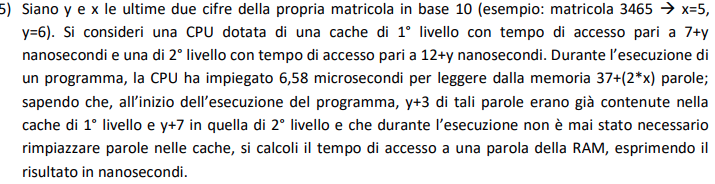
\includegraphics[width=1\linewidth]{es5_MiglioramentoPrestazioneMemoria}
	%\caption{}
	\label{fig:es5MiglioramentoPrestazioneMemoria}
\end{figure}

\textsf{{\small Non è mai stato necessario rimpiazzare parole nella cache = cache non variano.}} \\

$ \text{MATR} = 2602 \hspace{.1cm}(x = 2, y = 0) $ \\

$ \text{T}_\text{C1} = 7 \text{ ns} $ \\
$ \text{T}_\text{C2} = 12 \text{ ns} $ \\
$ \text{T}_\text{TOT} = 6,58 \overset{10^-6}{\text{ ms (millisecondi)}} = 6580 \overset{10^-9}{\text{ ns (nanosecondi)}} $ \\

$ \text{N}_\text{TOT} = 41 $ \\
$ \text{N}_\text{C1} = 3 $ \\
$ \text{N}_\text{C2} = 7 $ \\
$ \text{T}_\text{RAM} = ? $ \\

$ 6580 = 41 \cdot 7 + (41 - 3) \cdot 12 + (41 - 3 - 7) \cdot \text{T}_\text{RAM} $ \\
$ 6580 = 287 + 38 \cdot 12 + 31 \cdot \text{T}_\text{RAM} $ \\
$ 6580 = 287 + 456 + 31 \cdot \text{T}_\text{RAM} $ \\

$ \frac{6580 - 287 - 456}{31} = \text{T}_\text{RAM} $ \\

$ \text{T}_\text{RAM} = \frac{5837}{31} \simeq \color{red}\boxed{\normalcolor188,3 \text{ ns}} $ \\

% --- ESERCIZIO 6 MIGLIORAMENTO PRESTAZIONI MEMORIA ---

\newpage

\begin{figure}[ht]
	%\centering
	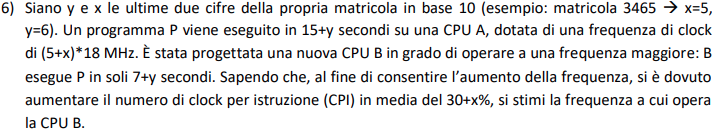
\includegraphics[width=1\linewidth]{es6_MiglioramentoPrestazioneMemoria}
	%\caption{}
	\label{fig:es6MiglioramentoPrestazioneMemoria}
\end{figure}

$ \text{MATR} = 2602 \hspace{.1cm}(x = 2, y = 0) $ \\

$ \text{T}_\text{A} = 15 \text{ s} $ \\
$ \text{F}_\text{A} = 126 \text{ Mhz} $ \\
$ \text{T}_\text{B} = 7 + y \text{ secondi} $ \\
$ \text{CPI}_\text{B} = 1,32 \cdot \text{CPI}_\text{A} $ \\
$ \text{F}_\text{B} = ? $ \\

\noindent\begin{minipage}{.5\linewidth}
\begin{equation*}
\begin{cases}
15 = \frac{1}{126 \cdot 10^6} \cdot \text{N}_\text{TOT} \cdot \widetilde{\text{CPI}_\text{A}} \\
7 = \frac{1}{\text{F}_\text{B}} \cdot \text{N}_\text{TOT} \cdot \widetilde{\text{CPI}_\text{B}} \\
\end{cases}
\end{equation*}
\end{minipage}
\begin{minipage}{.35\linewidth}
\begin{equation*}
	\begin{cases}
		15 \cdot 126 \cdot 10^6 = \text{N}_\text{TOT} \cdot \widetilde{\text{CPI}_\text{A}} \\
		7 \cdot \text{F}_\text{B} = \text{N}_\text{TOT} \cdot 1,32 \cdot \widetilde{\text{CPI}_\text{A}} \\
	\end{cases}
\end{equation*}
\end{minipage}

\begin{equation*}
\begin{cases}
1890 \cdot 10^6 = \text{N}_\text{TOT} \cdot \widetilde{\text{CPI}_\text{A}} \\
\text{F}_\text{B} = \frac{1890 \cdot 10^6 \cdot 1,32}{7} \\
\end{cases}
\end{equation*}

$ \text{F}_\text{B} \simeq 356,4 \cdot 10^6 \text{ hz} = \color{red}\boxed{\normalcolor 356,4 \text{ Mhz}} $ \\

% --- CONCLUSIONI ---

\newpage

\section{Conclusioni}

\flushright
\date{13, Dicembre 2020} \break

\centering

\textsf{{\normalsize In questo documento/articolo ho raccolto tutti o quasi gli esercizi svolti durante il corso di "Architetture degli Elaboratori" tranne alcuni che non ho scritto (come la Prova di Autovalutazione).}} \\

\textsf{{\normalsize Al momento ho concluso questo documento/articolo. \\ Ma in futuro, potreì aggiungere degli esercizi, in fondo, su tutti gli argomenti \\
		e poi le soluzioni a questi.}} \\
	
\textsf{{\normalsize Inoltre potreì anche mostrare i miei esercizi in Assembly che ho consegnato.}} \break


\flushleft
\large
%$ \mathfrak{Luca} $

\begin{comment}
\closing{Yours faithfully,\\
	\fromsig{\includegraphics[scale=1]{signature.jpg}} \\
	\fromname{Your name}
}
\end{comment}

%Le prime quattro non vanno, perchè il package emerald is not found
%JD: {\ECFJD\setul{0.1ex}{}\ul{~~John Quegpylf Doe~~}}

%Skeetch: {\ECFSkeetch\setul{0.1ex}{}\ul{~~John Quegpylf Doe~~}}

%Teen Spirit: {\ECFTeenSpirit\setul{-0.1ex}{0.3pt}\ul{~~John Quegpylf Doe~~}}

%Tall Paul: {\ECFTallPaul\setul{0.15ex}{}\ul{~~John Quegpylf Doe~~}}

Firma: {\cursive\setul{0.1ex}{}\ul{~~Luca~~}}

%Firma: {\iminfamily\setul{0.1ex}{}\ul{~~Luca~~}}

\end{document}
